\documentclass[11pt,a4paper]{article}
\usepackage[a4paper,margin=2.6cm]{geometry}
\usepackage{iftex}
\ifPDFTeX
  \usepackage[T2A]{fontenc}
  \usepackage[utf8]{inputenc}
  \usepackage[english,russian]{babel}
\else
  \usepackage{fontspec}
  \usepackage{polyglossia}
  \setdefaultlanguage{russian}
  \setotherlanguage{english}
  \defaultfontfeatures{Ligatures=TeX}
  % Font chain: local Times New Roman -> Liberation (Overleaf) -> CMU.
  \IfFontExistsTF{Times New Roman}{%
    \setmainfont{Times New Roman}%
    \setsansfont{Arial}%
    \setmonofont{Courier New}%
    \newfontfamily\cyrillicfont{Times New Roman}%
    \newfontfamily\cyrillicfontsf{Arial}%
    \newfontfamily\cyrillicfonttt{Courier New}%
  }{%
    \IfFontExistsTF{Liberation Serif}{%
      \setmainfont{Liberation Serif}%
      \setsansfont{Liberation Sans}%
      \setmonofont{Liberation Mono}%
      \newfontfamily\cyrillicfont{Liberation Serif}%
      \newfontfamily\cyrillicfontsf{Liberation Sans}%
      \newfontfamily\cyrillicfonttt{Liberation Mono}%
    }{%
      \setmainfont{CMU Serif}%
      \setsansfont{CMU Sans Serif}%
      \setmonofont{CMU Typewriter Text}%
      \newfontfamily\cyrillicfont{CMU Serif}%
      \newfontfamily\cyrillicfontsf{CMU Sans Serif}%
      \newfontfamily\cyrillicfonttt{CMU Typewriter Text}%
    }%
  }
\fi
% engine-agnostic English block: babel uses otherlanguage, polyglossia a named env
\ifPDFTeX
  \newenvironment{englishblock}{\begin{otherlanguage}{english}}{\end{otherlanguage}}
\else
  \newenvironment{englishblock}{\begin{english}}{\end{english}}
\fi
\usepackage{microtype}
\usepackage{mathtools,amssymb}
\usepackage{graphicx}
\usepackage{booktabs}
\usepackage{float}
\usepackage{caption}
\captionsetup{font=small,labelfont=bf}
\usepackage{enumitem}
\setlist{nosep,leftmargin=1.5em}
\usepackage{csquotes}
\usepackage[backend=biber,style=gost-numeric,sorting=none]{biblatex}
\addbibresource{../references_v2.bib}
\usepackage[unicode,hidelinks]{hyperref}
\setlength{\emergencystretch}{2em}

\title{{\normalsize\normalfont\hspace*{-\leftskip}\parbox{\linewidth}{\raggedright УДК~551.513}}\\[1.5em]
География сопряжённости иерархических уровней атмосферной циркуляции:\\
планетарная карта, её факторы и районирование}
\author{Н.~Сотириади\thanks{%
  \textbf{[ЗАПОЛНИТЬ ПЕРЕД ПОДАЧЕЙ]} организация, почтовый адрес с индексом, страна.\\
  E-mail: \texttt{n.sotiriadi@gmail.com}. ORCID: \textbf{[ЗАПОЛНИТЬ]}.}}
\date{2026}

\begin{document}
\maketitle

\begin{abstract}
Сопряжённость соседних масштабных уровней атмосферной циркуляции --- мера того, насколько размещение мезомасштабной изменчивости предопределено соседним крупным уровнем, --- в первой статье серии установлена как устойчивый региональный инвариант. Настоящая работа отвечает на собственно географический вопрос: какова планетарная география этого инварианта и чем она определяется. По полю относительного вихря реанализа ERA5 на поверхности 850~гПа построена глобальная мозаичная карта (936 ячеек по $\approx$667$\times$700~км, $60^\circ$~ю.\,ш.\,--\,$60^\circ$~с.\,ш., два сезона 2023~г.). Карта читается как физико-географическая: максимумы образуют сплошное кольцо штормовых путей Южного океана и северотихоокеанский и североатлантический штормовые пути, минимумы приурочены к очагам глубокой конвекции --- Амазонии, бассейну Конго и Индонезийскому архипелагу --- и к субтропическим муссонным землям. Сопряжённость монотонно растёт от экватора к умеренным широтам, над океаном выше, чем над сушей, во всех поясах, а в умеренных широтах Южного полушария выше, чем Северного, --- там, где штормовой путь не разорван материками. Сезонный ход в тропиках следует влажному сезону: сопряжённость ниже там и тогда, где активна муссонная конвекция. Статистическая атрибуция по заранее заявленным ковариатам подтверждает это прочтение: карта предсказуема вне подгонки ($R^2=0{,}40$--$0{,}54$, $p=0{,}001$), упорядочена практически одной осью --- активностью внетропических штормовых путей, --- при этом связь двухканальна (штормовая активность повышает сопряжённость через спектр, конвекция понижает сверх спектра), а стационарные условия территории сами по себе восстанавливают 90\,\% качества предсказания. Свободный модельный расчёт воспроизводит карту на 97\,\% достижимого согласия; воспроизводимый остаток атрибуции географически организован. Предложена типология территорий по организатору циркуляции и уровню сопряжённости --- основа районирования по устройству межуровневых связей.

\smallskip
\noindent\textbf{Ключевые слова:} региональная география, физико-географическое районирование, сопряжённость масштабов, атмосферная циркуляция, штормовые пути, конвективный режим, муссон, реанализ, атрибуция.
\end{abstract}

\begin{englishblock}
\begin{abstract}
\noindent\textbf{Geography of the coupling between hierarchical levels of the atmospheric
circulation: a planetary map, its controls and a regionalisation}

\smallskip\noindent N.~Sotiriadi

\smallskip\noindent The coupling of neighbouring scale levels of the atmospheric circulation
--- a measure of how far the placement of mesoscale variability is set by the adjacent large
level --- was established in the first paper of this series as a stable regional invariant.
The present paper asks the properly geographical question: what is the planetary geography of
this invariant and what governs it. From the ERA5 relative-vorticity field at 850~hPa a global
mosaic map is built (936 tiles of $\approx$667$\times$700~km, $60^\circ$S--$60^\circ$N, two
seasons of 2023). The map reads as a physical-geographical one: the maxima form the continuous
storm-track ring of the Southern Ocean and the North Pacific and North Atlantic storm tracks;
the minima sit over the deep-convective cores --- Amazonia, the Congo basin and the Maritime
Continent --- and over the subtropical monsoon lands. Coupling rises monotonically from the
equator to mid-latitudes, is higher over ocean than over land in every belt, and is higher in
the Southern than in the Northern mid-latitudes, where the storm track is not broken by
continents. The tropical seasonal cycle follows the wet season: coupling is lower where and
when monsoon convection is active. Statistical attribution on pre-declared covariates confirms
this reading: the map is predictable out of sample ($R^2=0.40$--$0.54$, $p=0.001$), is ordered
by essentially one axis --- extratropical storm-track activity --- while the association is
two-channel (storm activity raises coupling through the spectrum, convection lowers it beyond
the spectrum), and stationary boundary conditions alone recover 90\,\% of the predictive skill.
A free-running model integration reproduces the map at 97\,\% of the attainable agreement; the
reproducible attribution residual is geographically organised. A typology of territories by
circulation organiser and coupling level is proposed as a basis for regionalisation by the
architecture of inter-level links.

\smallskip
\noindent\textbf{Keywords:} regional geography, physical-geographical regionalisation, scale
coupling, atmospheric circulation, storm tracks, convective regime, monsoon, reanalysis,
attribution.
\end{abstract}
\end{englishblock}

\section{Введение}
\label{sec:intro}

\subsection{От регионального инварианта к его географии}

Региональная дифференциация атмосферной циркуляции традиционно описывается климатологией её ведущих организаторов: внетропических штормовых путей --- полос повышенной повторяемости и интенсивности циклонических возмущений умеренных широт \cite{HoskinsValdes1990,Chang2002,HoskinsHodges2005,Shaw2016} --- и режимов глубокой конвекции тропиков и муссонных областей \cite{Houze2004,Feng2021}. В первой статье серии\footnote{Сотириади~Н. Сопряжённость иерархических уровней атмосферной циркуляции как региональный инвариант (первая статья настоящей серии; подана в печать). Протоколы, код и численные результаты обеих работ открыты в едином репозитории: \url{https://github.com/Theclimateguy/Shroedinger}.} к этому описанию добавлена характеристика иного типа: по полю относительного вихря на поверхности 850~гПа построен профиль сопряжённости соседних октавных уровней~$P$ --- мера того, насколько размещение мезомасштабной изменчивости предопределено соседним крупным уровнем. Показано, что эта величина удовлетворяет операциональному определению инварианта динамики геосистем \cite{Puzachenko1986,Puzachenko2004,Puzachenko2010} в традиции выделения уровней организации регионального климата \cite{Krenke2019}: устойчива к смене сезона, года, фазы Эль-Ниньо~--- Южного колебания (ЭНСО), источника данных (MERRA-2 \cite{Gelaro2017}) и схемы разбиения территории, содержит воспроизводимую информацию сверх спектра поля и воспроизводится в модельном расчёте без усвоения наблюдений. Обоснование конструкции, операциональное описание процедуры и каталог отвергнутых интерпретаций даны там же и здесь не повторяются.

\emph{Терминологическая оговорка, определяющая всё дальнейшее чтение.} Величина~$P$ измеряет \emph{пространственную со-организацию} активности соседних масштабных уровней --- то, насколько согласованно они размещены по территории. Слово <<сопряжённость>> служит кратким именем этого факта и не подразумевает ни динамической связи между масштабами, ни переноса энергии: обе интерпретации прямо проверены и отвергнуты в первой статье. Поэтому везде, где ниже говорится о том, что режим <<повышает>> либо <<понижает>> сопряжённость, имеется в виду устойчивая статистическая связь заданного знака, а не установленный физический процесс.

Настоящая работа ставит следующий, собственно географический вопрос: \emph{какова планетарная география инварианта и чем она определяется} --- в каких отношениях его карта находится с известными организаторами циркуляции и с экзогенными граничными условиями территории. Рабочая рамка --- цепочка <<географическая конфигурация $\to$ организация атмосферных процессов $\to$ сопряжённость уровней>>: конфигурация материков, океанов и горных систем задаёт, где складываются штормовые пути и конвективные режимы, а их организация проявляется в устройстве межуровневых связей. Слово <<географический>> употребляется при этом в трёх различимых смыслах: \emph{географическое положение} (широта, долгота); \emph{физико-географические свойства территории} (рельеф, соотношение суши и моря, изрезанность берега, температура поверхности океана); \emph{тип циркуляционного режима над территорией} (штормовые пути, конвективный режим). Первые два смысла отсылают к условиям, экзогенным по отношению к циркуляции, третий --- к состоянию, складывающемуся вместе с ней. Постановка продолжает отечественную традицию выделения уровней организации геосистем и физико-географического районирования \cite{Sochava1978,Isachenko1991,Bertrand1968} и примыкает к общему для наук о Земле вопросу о масштабе, на котором территория обладает собственной организацией \cite{Simon1962,Levin1992,WuLoucks1995}.

Первая попытка атрибуции была предпринята на региональной выборке и закончилась неудачей: на двенадцати региональных скалярах пять средовых ковариат дали при перекрёстной проверке с исключением по одному отрицательную объяснённую дисперсию ($R^2_{\mathrm{LOO}}=-0{,}62$, $p=0{,}65$). Урок методический: двенадцать точек не способны корректно вместить ни одно семейство ковариат. Решение --- смена единицы выборки: переход к мозаичной карте, где единицей выступает ячейка мозаики (далее --- тайл) размером в сотни километров, а региональная принадлежность тайлов служит блокирующим фактором статистики. Число степеней свободы растёт на порядок ($n\approx144$, затем $n\approx936$), межрегиональные смешения контролируются выбыванием целых регионов или секторов долготы.

Задачи работы: (1)~построить глобальную мозаичную карту тонкомасштабного~$P$ с суррогатной поправкой и дать её географическое описание --- широтный ход, полушарную асимметрию, контраст суши и океана, сезонность; (2)~выполнить статистически корректную атрибуцию географии карты по заранее заявленным внешним ковариатам, с отрицательным контролем и контрольной мишенью, и описать географию остатка; (3)~проверить природу карты сопоставлением со свободным модельным расчётом; (4)~предложить типологию территорий по организатору циркуляции и уровню сопряжённости как основу районирования; (5)~замкнуть атрибуцию со стороны времени --- атрибутировать тропический избыток межгодовой изменчивости по заранее названным климатическим индексам и проверить гипотезу статичности инварианта.

\subsection{Три объяснения географии и гипотеза статичности}
\label{sec:hypotheses}

Вопрос о географии карты~$P$ распадается на выбор между тремя объяснениями, каждое из которых имеет собственное проверяемое следствие; гипотезы и распределение ковариат по ярусам зафиксированы протоколом до вычислений.

\emph{H1, экзогенная.} География~$P$ определяется стационарными граничными условиями территории --- рельефом, конфигурацией суши и океана, широтой, полем температуры поверхности океана. Следствие: карта предсказуема по одному ярусу~1, а характеристики циркуляционного режима не добавляют к предсказанию существенного.

\emph{H2, циркуляционная.} География~$P$ определяется состоянием циркуляции --- активностью внетропических штормовых путей и конвективным режимом. Следствие: ведущие нагрузки принадлежат ярусу~2, и связь сохраняется \emph{внутри} климатически однородных областей, где экзогенные условия почти постоянны.

\emph{H3, артефактная.} Карта~$P$ --- свойство наблюдательной сети и системы усвоения, а не атмосферы. Следствие: карта не должна воспроизводиться расчётом, не усваивающим атмосферных наблюдений.

H1 и H2 не исключают друг друга: если экзогенная конфигурация задаёт, \emph{где} располагаются циркуляционные режимы, то оба яруса будут читать одну и ту же карту, и содержательным результатом окажется мера их совместности. Поэтому проверка измеряет вклад каждого яруса по отдельности: разделение ковариат по ярусам, корреляции внутри регионов, нуль-модель, сохраняющая зональную структуру, и сопоставление со свободным расчётом. Решающие правила зафиксированы протоколами \emph{до} вычислений (табл.~\ref{tab:hyp}).

Наконец, $P$ заявлен в первой статье как \emph{статичный} инвариант сложившегося режима --- характеристика установившейся организации, а не переменная с собственной динамикой. Отсюда проверяемое следствие: при перестройке режима величина не должна опережать перестройку и превосходить по чувствительности стандартные показатели среднего поля (разд.~\ref{sec:time}). Работа остаётся в рамках эмпирического картирования, атрибуции и районирования; интерпретирующая рамка вынесена в третью статью серии.

\section{Материалы и методы}
\label{sec:data}

\subsection{Данные и две части протокола}

Материал --- реанализ ERA5 \cite{Hersbach2020,Soci2024}: составляющие ветра на изобарической поверхности 850~гПа, сетка $0{,}25^\circ$, шаг 6~ч, поле относительного вихря --- идентично первой статье серии. Обе части выполнены по единому протоколу, зафиксированному до вычислений (все критерии, пороги и нуль-модели заданы заранее; отступления фиксировались в журнале протокола).

\emph{Часть~A} --- 144 тайла внутри двенадцати равновеликих областей первой статьи (12 областей $\times$ 12 тайлов): сетка $3\times4$ на область, ячейки $\approx667\times700$~км; использованы только поля, уже имевшиеся в архиве программы (сезонные окна 2021--2024~гг.). \emph{Часть~B} --- глобальная сетка из 936 тайлов: широтные полосы по $6^\circ$ ($\approx$667~км), долготные ячейки по 700~км на центральной широте полосы (точное кольцевое покрытие без остатка), пояс $60^\circ$~ю.\,ш.\,--\,$60^\circ$~с.\,ш.; два независимых сезона --- январь--март и июль--сентябрь 2023~г. Из анализа исключены 34 тайла со средней высотой рельефа более 1200~м (поверхность 850~гПа ниже подстилающей); в описании и атрибуции участвуют 902 тайла.

\emph{Целевая величина} --- тонкомасштабный профиль~$P$ с суррогатной поправкой: сопряжённость огибающих на лестнице 50--100--200--400~км (три ступени), вычисленная по внутренней маске тайла и взятая в превышении над медианой 99 фазовых суррогатов, генерируемых отдельно для каждой пары <<тайл--окно>>. Операторы уровня и огибающей, форма корреляции, маска и построение суррогатов идентичны первой статье и здесь не пересказываются.

Диапазон 50--400~км выбран по двум причинам. Геометрическая: внутренняя маска отсекает краевую полосу шириной $\min(2\ell_{\max};\,0{,}25$ размера тайла$)$, и при тайле $\approx667\times700$~км ступень 400--800~км внутренней области уже не оставляет. Содержательная: диапазон охватывает переход от мезомасштаба~$\beta$ к мезомасштабу~$\alpha$, где различие режимов штормовых путей и влажной конвекции выражено в первой статье наиболее чисто. Эти полосы частично лежат ниже эффективного разрешения реанализа (125--220~км по правилу 4--7 шагов сетки \cite{Skamarock2004}; 500--600~км по спектральной оценке \cite{Bolgiani2022}). Работа с ними корректна по трём причинам: суррогатная поправка сравнивает поле с полем той же спектральной структуры, прошедшим тот же вычислительный тракт; карта воспроизводится свободным расчётом другой конфигурации модели на 97\,\% достижимого согласия (разд.~\ref{sec:model}); мозаичная карта согласована с региональным уровнем первой статьи ($\rho=0{,}874$), где эффект выдерживает контроль по разрешённым ступеням. Остающееся ограничение обсуждается в разд.~\ref{sec:limitations}.

\subsection{Ковариаты и их причинный статус}

Внешние ковариаты разбиты на два яруса, и граница между ними задана протоколом \emph{до} вычислений --- она определяет допустимый язык интерпретации, а не подбирается под результат.

\emph{Ярус~1 --- экзогенные граничные условия} (допустим направленный язык <<формируют>>): средняя высота рельефа в тайле и его расчленённость (стандартное отклонение высоты); доля суши; контрастность подстилающей поверхности суша--море (стандартное отклонение маски суши внутри тайла --- мера изрезанности берега); модуль широты; средний модуль градиента температуры поверхности океана (ТПО). Основания стандартны: рельеф --- барьерный отклик потока, доля суши и контрастность берега --- контраст нагрева и место заложения приземных фронтальных зон, модуль широты --- радиус деформации, градиент ТПО --- бароклинность нижней тропосферы над океаном.

\emph{Ярус~2 --- совместно складывающиеся характеристики состояния} (только язык совместной организации, без направленности): климатология конвективной доступной потенциальной энергии CAPE за 2021--2024~гг. \cite{RiemannCampe2009} --- показатель конвективного режима территории --- и синоптическая кинетическая энергия вихрей (дисперсия ветра относительно скользящего 5-суточного среднего; далее --- вихревая энергия) --- стандартная мера активности внетропических штормовых путей, восходящая к классическим полосовым климатологиям синоптической изменчивости \cite{Blackmon1976,HoskinsHodges2005,HoskinsHodges2019}.

\emph{Отрицательный контроль} --- индекс листовой поверхности (климатология ERA5, сумма компонент низкой и высокой растительности): биологический показатель, механистически неправдоподобный как фактор сопряжённости масштабов 50--400~км на уровне 850~гПа. Ожидаемый исход --- отсутствие прироста предсказания.

\subsection{Статистический дизайн}

\emph{Нуль-модели атрибуции.} В части~A нуль строится перестановками региональных меток целыми блоками тайлов (999 повторов): тайлы одного региона перемещаются вместе, поэтому внутрирегиональная зависимость сохраняется. В части~B нуль --- циклический поворот долготной сетки ковариат относительно карты~$P$ на случайный сдвиг не менее $30^\circ$ (999 повторов). Поворот сохраняет пространственную автокорреляцию обоих полей и, поскольку модуль широты инвариантен относительно поворота долготы, всю зональную структуру целиком: значимость теста удостоверяет именно \emph{незональную} часть атрибуции --- привязку карты к фактическому положению штормовых путей и конвективных очагов.

\emph{Проверка предсказания и эффективная размерность.} Предсказание проверяется выбыванием целыми блоками --- по региону (часть~A) либо по одному из шести секторов долготы по $60^\circ$ (часть~B); сообщаемое $R^2$ всегда относится к предсказанию на не участвовавших в подгонке блоках. Эффективная размерность оценивается прямым пошаговым отбором ковариат с тем же блочным выбыванием; $k_{80}$ --- число ковариат, достаточное для 80\,\% полного качества.

\emph{Потолок надёжности карты} --- внутрисезонное расщепление выборки пополам: сроки каждой пары <<тайл--сезон>> делятся по чётности на две непересекающиеся половины, каждая половина привязывается к собственным 99 суррогатам, надёжность полной выборки восстанавливается поправкой Спирмена--Брауна \cite{Spearman1910,Brown1910}. \emph{Контрольная (плацебо) мишень} --- наклон пространственного спектра тайла: если бы атрибуция~$P$ лишь повторяла атрибуцию спектра, нагрузки двух мишеней совпадали бы.

\subsection{Описательные характеристики карты и типология}

В отличие от атрибуции, географическое описание карты (разд.~\ref{sec:geo}) и типология территорий (разд.~\ref{sec:region}) не подчинены решающим правилам и не сопровождаются проверкой значимости: это \emph{описательный} слой, построенный по уже вычисленным и зафиксированным тайловым значениям. Широтный ход --- средние по полосам $6^\circ$; контраст суши и океана --- по доле суши в тайле (порог 0,5); сезонность --- разность карт января--марта и июля--сентября. Типология задана двумя осями с глобальными терцилями по 902 тайлам: \emph{организатор циркуляции} --- <<штормовой путь>>, если вихревая энергия тайла не ниже верхней терцили, <<конвективный режим>>, если не ниже верхней терцили климатология CAPE (при выполнении обоих условий --- по большему рангу), иначе <<без ведущего организатора>>; \emph{уровень сопряжённости} --- нижняя, средняя или верхняя терциль двухсезонного среднего~$P$. Отдельно помечены тайлы, граничащие с исключёнными по орографии: их значения следует читать с осторожностью.

\section{Планетарная карта: географическое описание}
\label{sec:geo}

\subsection{Общий рисунок и его провинции}
\label{sec:map}

Центральный объект работы --- глобальная карта тонкомасштабного~$P$ с суррогатной поправкой (рис.~\ref{fig:global}), построенная по 902 тайлам пояса $60^\circ$~ю.\,ш.\,--\,$60^\circ$~с.\,ш. и двум сезонам 2023~г. Среднее по карте 0,263 при стандартном отклонении 0,042 и размахе от 0,10 до 0,41. Прежде всякой статистики её стоит прочесть как карту.

Максимумы образуют узнаваемую циркуляционную географию. Первая провинция --- \emph{сплошное кольцо Южного океана} между $40$ и $60^\circ$~ю.\,ш.: значения 0,35--0,37 по всей длине кольца, пик 0,41 к югу от Новой Зеландии, в Тасмановом секторе. Вторая --- \emph{штормовые пути Северного полушария}: залив Аляски (0,37), море Лабрадор и Гудзонов залив, Норвежское море (0,35--0,36) --- в точности те пояса, где внетропическая бароклинная активность организует поле сразу на нескольких масштабах \cite{HoskinsValdes1990,Chang2002,HoskinsHodges2005,Shaw2016}. Третья, более локальная, --- \emph{побережья с сильными градиентами температуры поверхности}: калифорнийское и центральночилийское (0,36), тихоокеанское побережье Центральной Америки; к ней же примыкает область к югу от Явы (0,38), единственный тропический океанический тайл в верхней двадцатке.

Минимумы столь же узнаваемы и распадаются на три типа. Первый --- \emph{экваториальные очаги глубокой конвекции}: западная Амазония (0,16--0,18), бассейн Конго (0,18), Борнео (0,15) \cite{NealeSlingo2003,Feng2021}. Второй --- \emph{субтропические муссонные земли и побережья}: Южный Китай (0,10--0,15; абсолютный минимум карты), побережья Красного моря и Аравии (0,14--0,18). Третий --- \emph{предгорья и подветренные зоны крупных горных систем}: Чако и Андское предгорье, окраина Мексиканского нагорья, Иранское нагорье, Западная Анатолия, Патагония. Тайлы третьего типа граничат с орографическим исключением (91 такой тайл на карте; их среднее 0,253 против 0,264 у остальных), и четверть нижнего дециля карты приходится именно на них; единичные экстремумы здесь ненадёжны. Промежуточные значения занимают субтропические океаны и внутриматериковые области умеренного пояса.

Таким образом, первое прочтение карты --- содержательно географическое: она разделяет территории по типу господствующего циркуляционного режима, а не по климатическому поясу. Описательное разложение дисперсии подтверждает это: 51\,\% приходится на широтные полосы по $6^\circ$, 10\,\% --- на долготные секторы внутри полос, 39\,\% --- на изменчивость внутри ячеек $6^\circ\times60^\circ$. Почти половина рисунка незональна, и именно эта половина различает конкретные территории.

\begin{figure}[t]
\centering
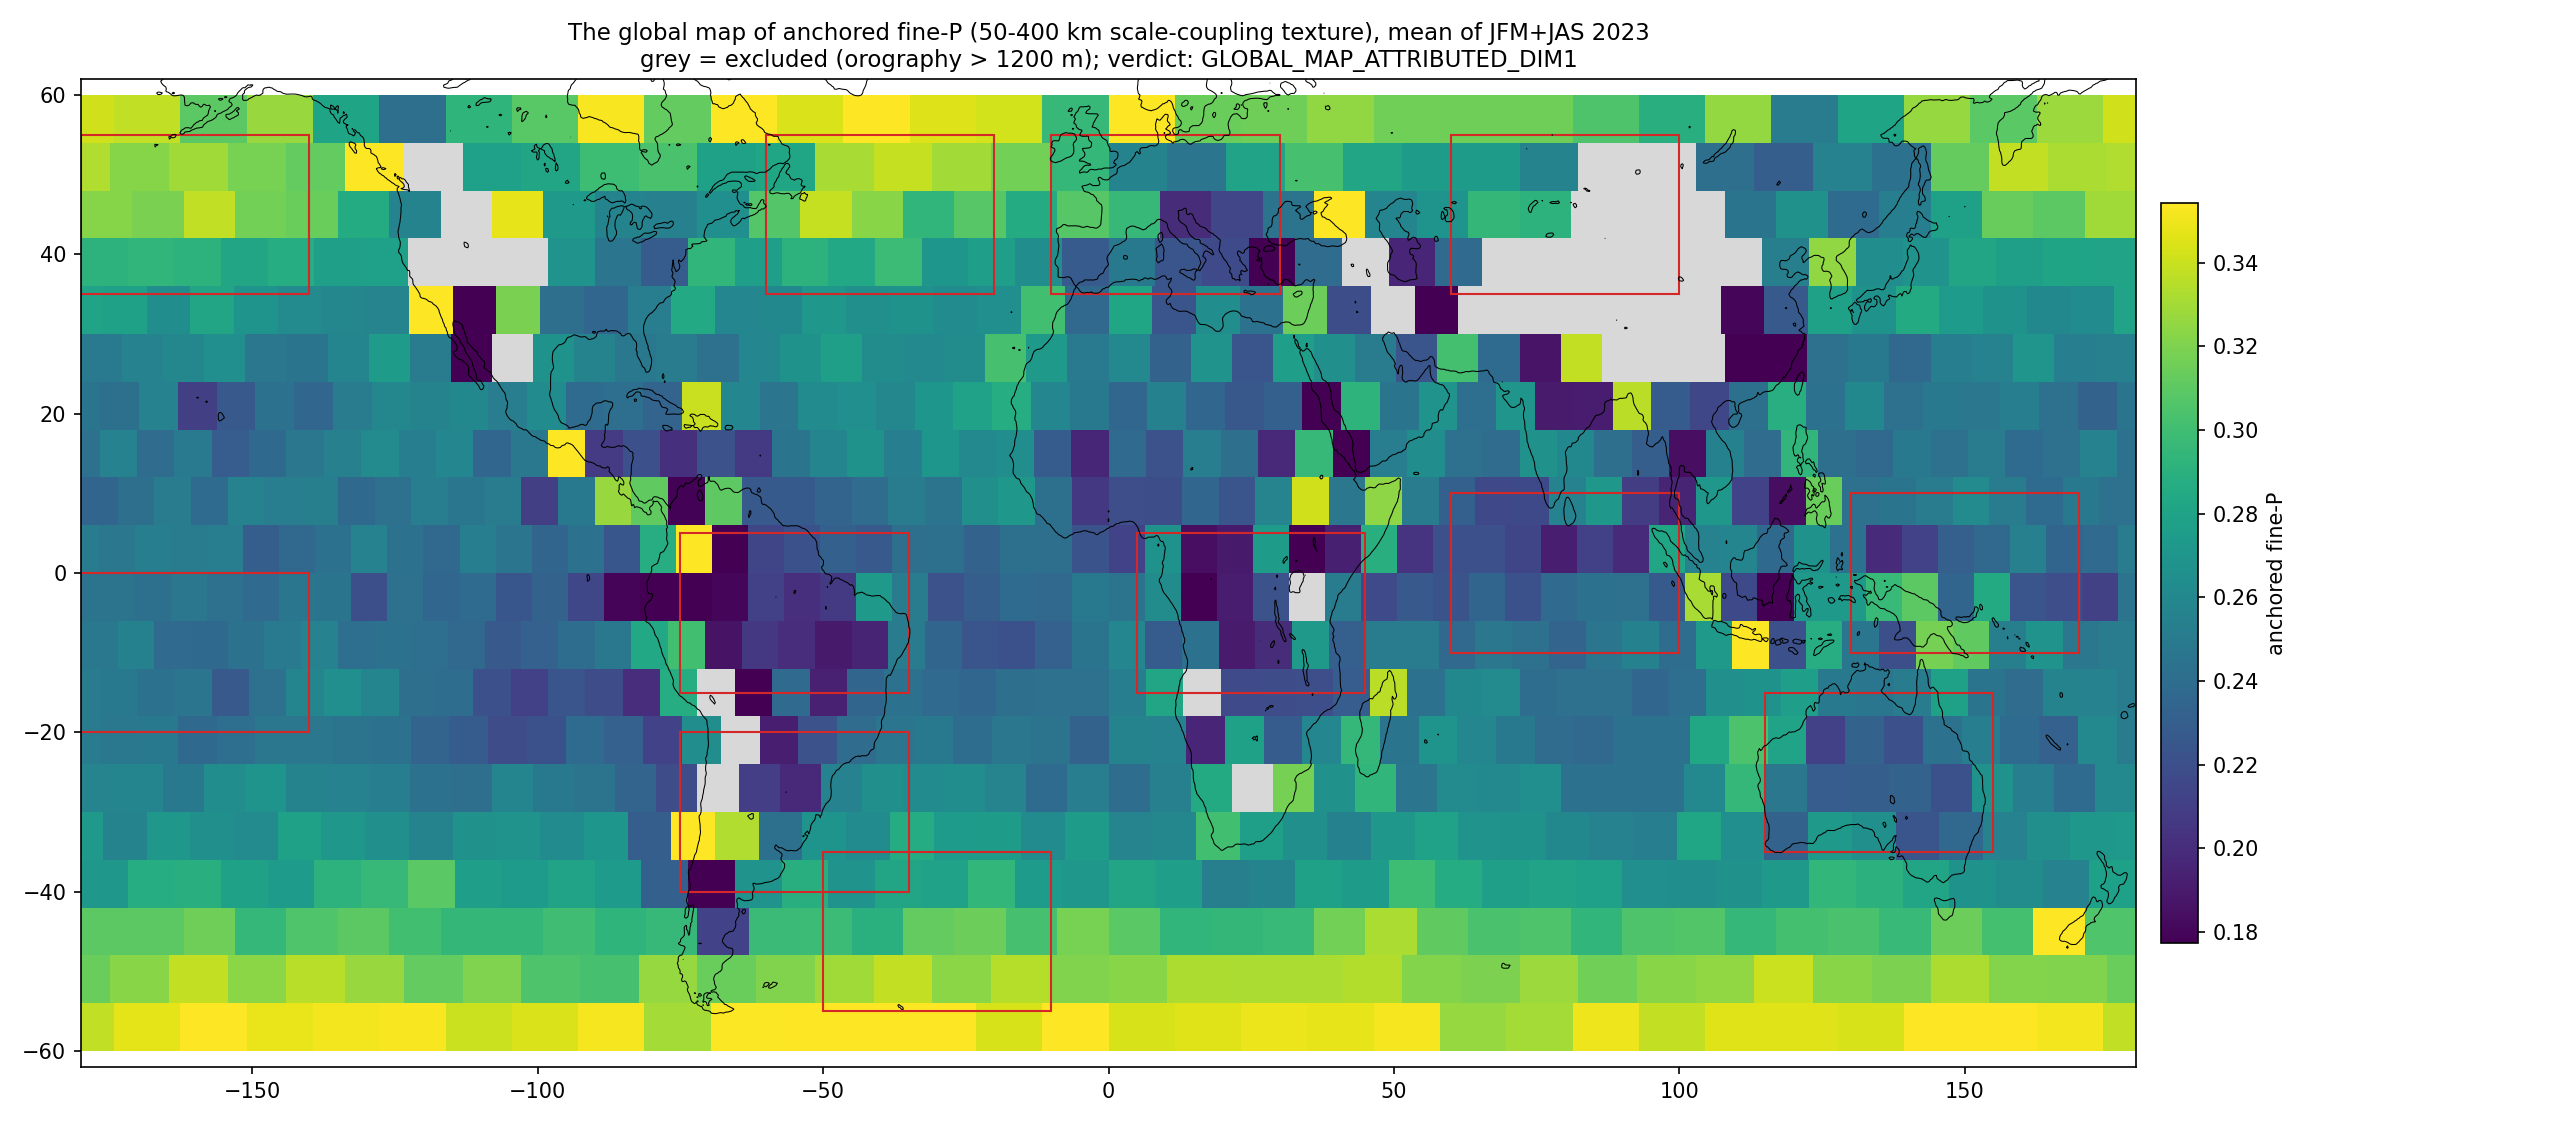
\includegraphics[width=\linewidth]{figures/fig2_global_map.png}
\caption{Глобальная карта тонкомасштабного $P$ с суррогатной поправкой (сопряжённость полос 50--400~км), среднее сезонов январь--март и июль--сентябрь 2023~г., 936 тайлов, $60^\circ$~ю.\,ш.\,--\,$60^\circ$~с.\,ш. Серым --- тайлы, исключённые по орографии (средняя высота более 1200~м); красные рамки --- двенадцать областей программы. Максимумы --- кольцо штормовых путей Южного океана, северотихоокеанский и североатлантический штормовые пути; минимумы --- Амазония, бассейн Конго, Индонезийский архипелаг и субтропические муссонные земли.}
\label{fig:global}
\end{figure}

\subsection{Широтный ход и полушарная асимметрия}

Широтный ход карты (рис.~\ref{fig:zonal},~а) монотонен: от 0,233 на экваторе через плоское плато 0,24--0,25 в тропиках до 0,26--0,27 на $33^\circ$, 0,29--0,30 на $45^\circ$ и 0,32--0,35 на $57^\circ$. Рост начинается там, где начинаются штормовые пути, и продолжается до края области анализа; тропики в среднем однородны, и вся их география --- незональная.

Полушария симметричны до $27^\circ$ (разность средних не превышает 0,005), а далее расходятся (рис.~\ref{fig:zonal},~б): Южное полушарие опережает Северное на 0,008 при $33^\circ$, на 0,016 при $45^\circ$ и на 0,03 при $51$--$57^\circ$. Асимметрия имеет два слагаемых. Часть её --- доля суши: в Северном полушарии на широтах $45$--$57^\circ$ половина тайлов приходится на материки, в Южном --- ни одного. Но и при сравнении только океанических тайлов Южное полушарие остаётся выше (0,348 против 0,333 на $57^\circ$): кольцо Южного океана организовано сильнее северных штормовых путей и на равной подстилающей поверхности. Это согласуется с классической климатологией штормовых путей: южный путь непрерывен по кругу широты и не разорван материками и горными барьерами, тогда как северные пути локализованы в двух океанических бассейнах и ослабевают над Евразией и Северной Америкой \cite{Trenberth1991,HoskinsHodges2005}.

\begin{figure}[t]
\centering
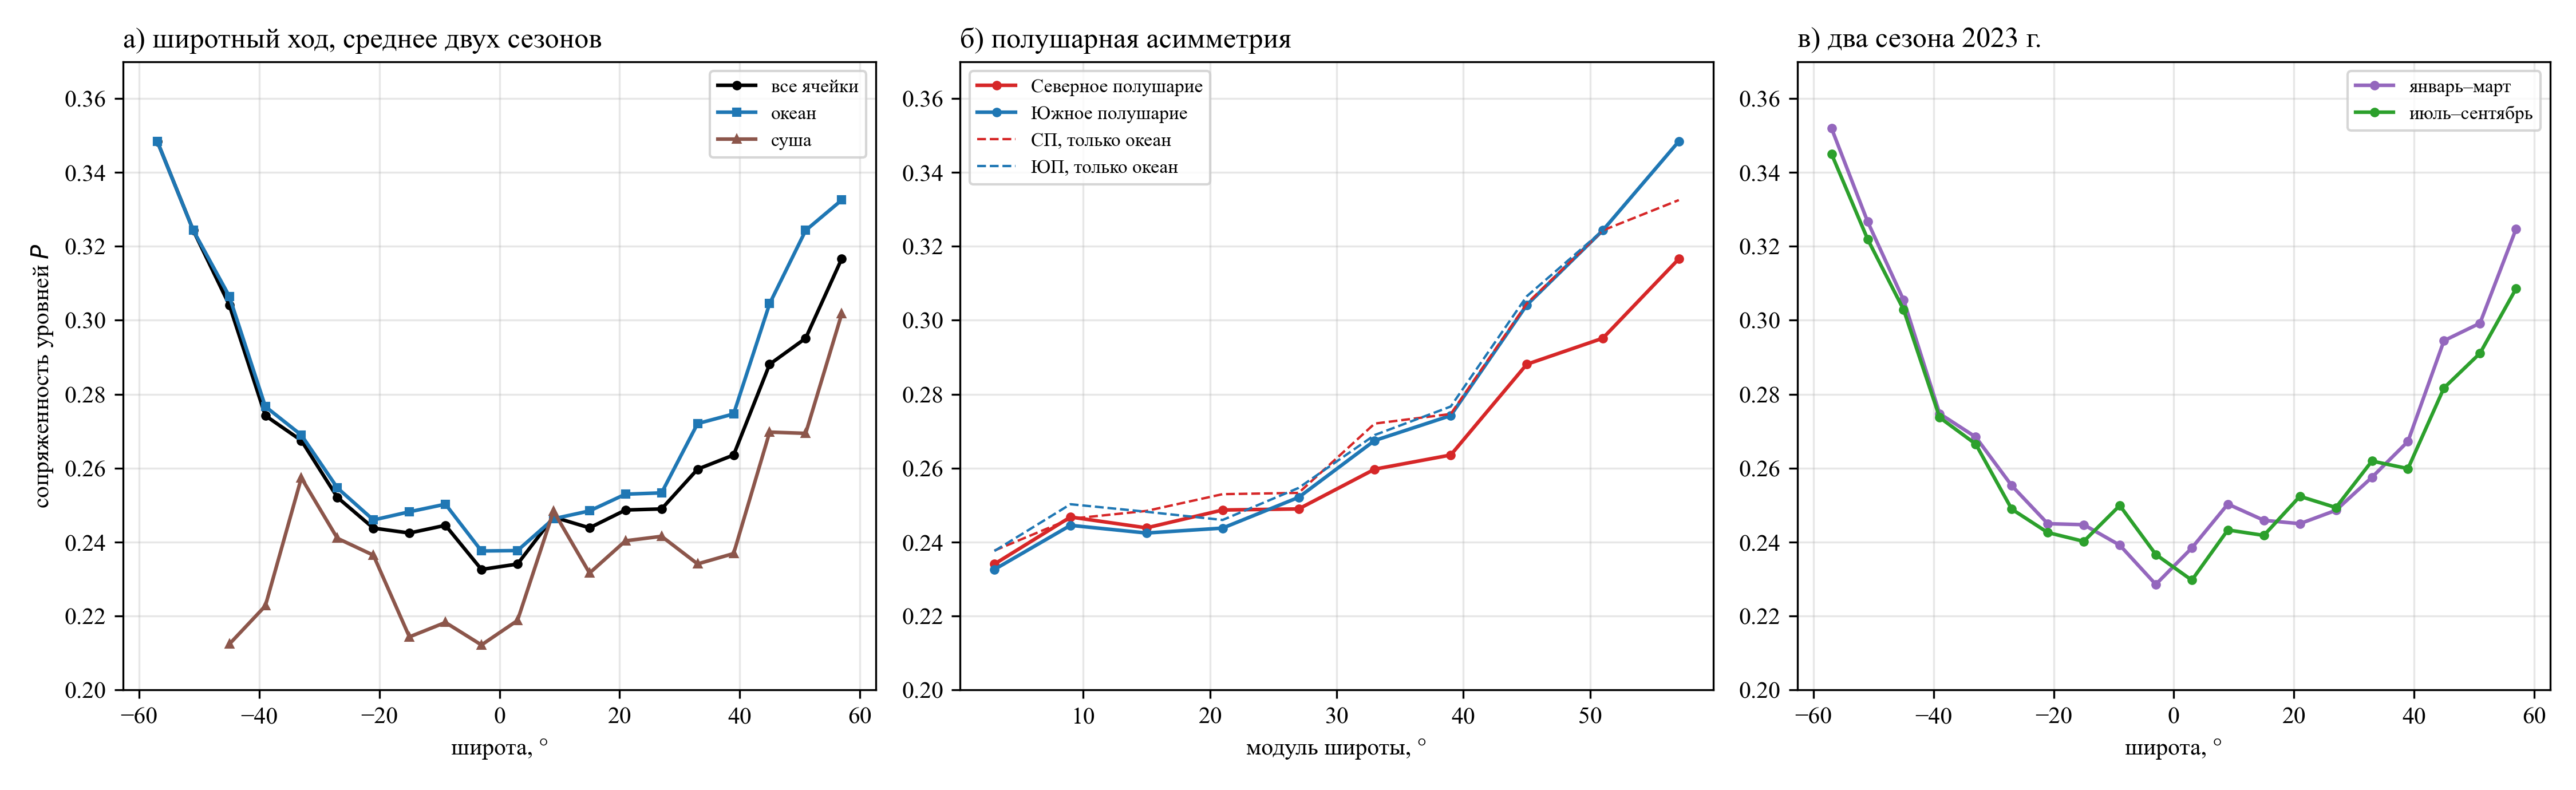
\includegraphics[width=\linewidth]{figures/fig2_zonal_profiles.png}
\caption{Широтная структура карты (описательно, 902 тайла): а~--- средние по полосам $6^\circ$ для всех тайлов, океанических (доля суши $<0{,}5$) и материковых (доля суши $\ge0{,}5$), среднее двух сезонов 2023~г.; б~--- те же средние по модулю широты для Северного и Южного полушарий (сплошные линии --- все тайлы, штриховые --- только океан); в~--- широтный ход для сезонов январь--март и июль--сентябрь.}
\label{fig:zonal}
\end{figure}

\subsection{Суша и океан}

Над океаном сопряжённость выше, чем над сушей, во всех поясах: 0,243 против 0,226 в тропиках ($0$--$15^\circ$), 0,255 против 0,237 в субтропиках ($15$--$35^\circ$), 0,309 против 0,270 в умеренных широтах ($35$--$60^\circ$); по карте в целом --- 0,269 против 0,244. Контраст растёт к умеренным широтам вместе с ростом самой величины и там достигает 0,04 --- порядка стандартного отклонения всей карты. Два обстоятельства заслуживают внимания. Во-первых, контраст не сводится к рельефу: тайлы с высотой более 1200~м исключены, а среди оставшихся материковых тайлов умеренного пояса преобладают равнины. Во-вторых, в тропиках материковые тайлы --- это как раз очаги глубокой конвекции, и здесь контраст суши и океана есть контраст конвективного и неконвективного режима, а не подстилающей поверхности как таковой; разделить два прочтения на описательном уровне нельзя, и это одна из задач атрибуции (разд.~\ref{sec:why}).

\subsection{Сезон: штормовые пути и муссоны}

Карта сезонно устойчива: медиана модуля разности между картами января--марта и июля--сентября составляет 0,016 при 90-м перцентиле 0,048 (рис.~\ref{fig:zonal},~в; рис.~\ref{fig:seasons}). Систематическая сезонность невелика и имеет ясную географию. В умеренных широтах Северного полушария зимняя карта выше летней на 0,011 --- в согласии с зимним максимумом активности северных штормовых путей; в Южном полушарии сезонный контраст умеренных широт втрое меньше (0,004), что отвечает слабой сезонности южного штормового пути \cite{Trenberth1991}.

В тропиках и субтропиках знак сезонного изменения следует \emph{влажному сезону}: над материками Северного полушария ($0$--$25^\circ$~с.\,ш.) сопряжённость в январе--марте выше, чем в июле--сентябре, на 0,017, над материками Южного ($0$--$25^\circ$~ю.\,ш.) --- ниже на 0,012. Иначе говоря, сопряжённость понижается там и тогда, где активна муссонная конвекция. Крупнейшие сезонные сдвиги карты (0,10--0,18) приходятся на муссонные земли: льяносы Колумбии и Венесуэлы, Сахель и Эфиопское предгорье, Малабарское побережье Индии, побережье Гвинейского залива --- с понижением летом Северного полушария; Новая Гвинея, Сулавеси, Тимор, Восточная Африка к югу от экватора --- с понижением летом Южного. Рисунок не без исключений (Японские острова и Западный Судан понижаются зимой Северного полушария), но в среднем по материкам он выдерживается. Сезонная география, следовательно, повторяет пространственную: тот же конвективный режим, который задаёт минимумы карты в Амазонии и Конго, задаёт и её сезонное понижение в муссонных областях.

\begin{figure}[t]
\centering
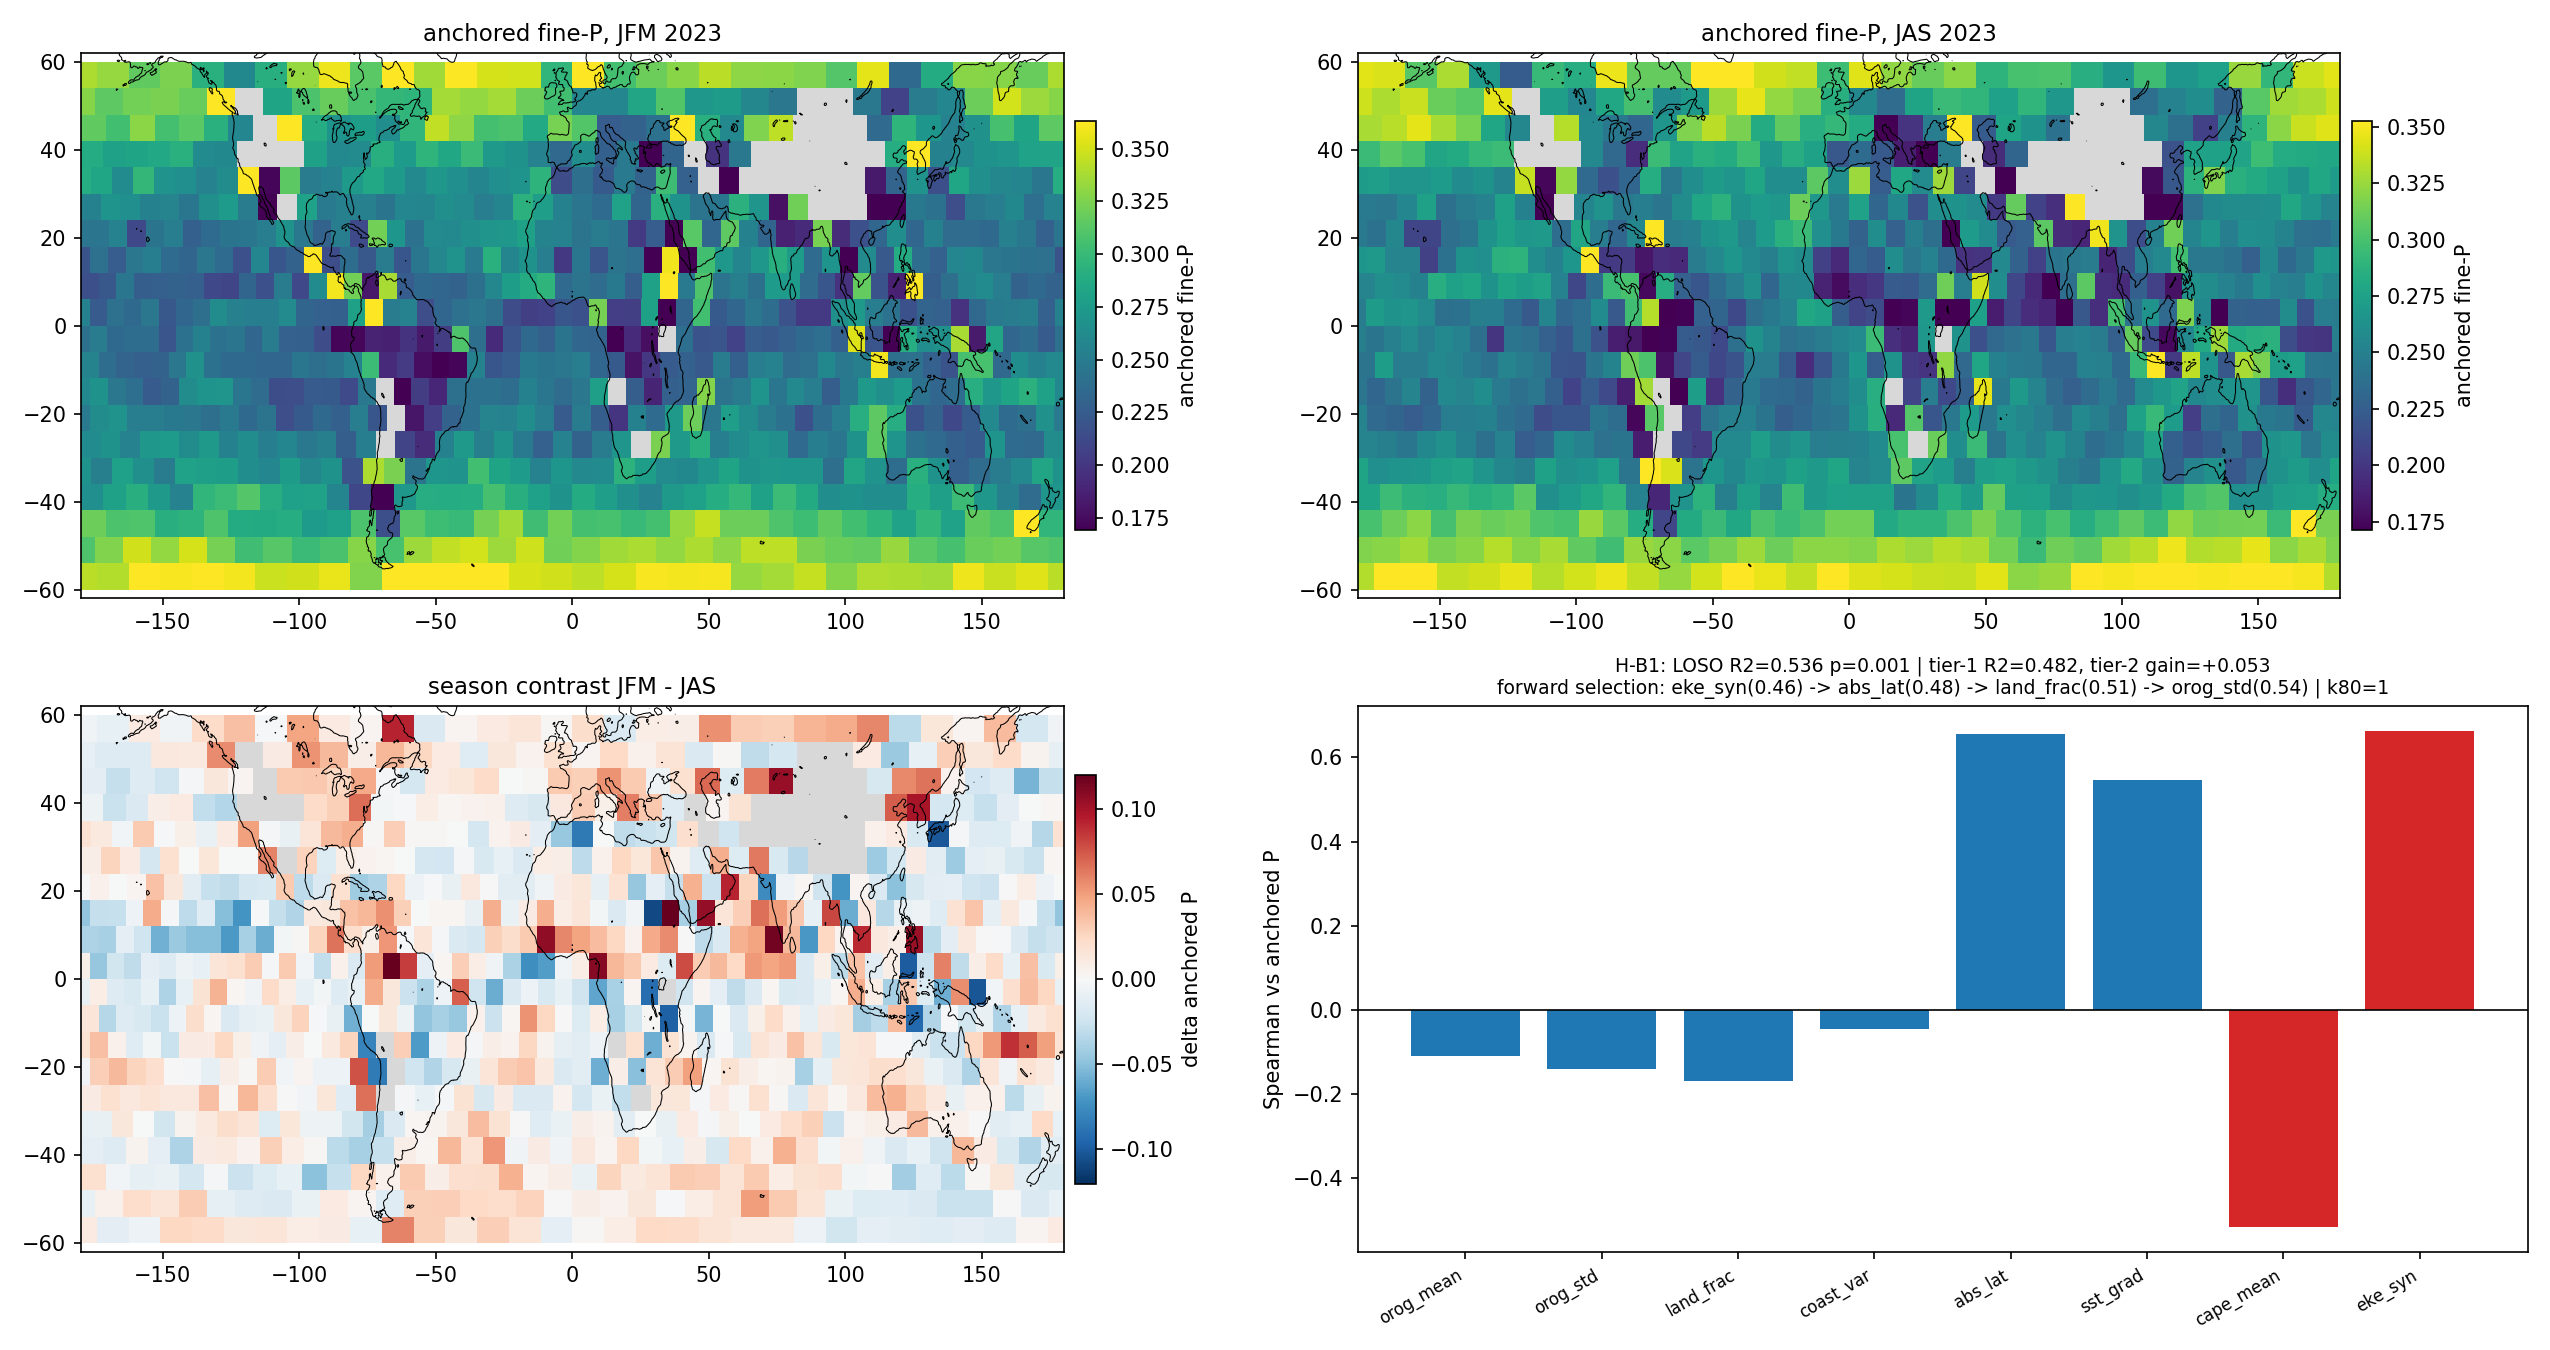
\includegraphics[width=\linewidth]{figures/fig2_seasons_attribution.png}
\caption{Сезонная структура и атрибуция глобальной карты: карты $P$ (с суррогатной поправкой) по сезонам январь--март и июль--сентябрь 2023~г. (вверху), сезонный контраст (внизу слева; медиана модуля 0,016) и нагрузки восьми ковариат с кривой пошагового отбора (внизу справа): вихревая энергия одна даёт $R^2=0{,}456$ из полных $0{,}536$.}
\label{fig:seasons}
\end{figure}

\section{Почему карта такая: факторы географии}
\label{sec:why}

Описание разд.~\ref{sec:geo} подсказывает объяснение --- штормовые пути и конвекция, --- но не проверяет его: широтный ход, контраст суши и океана и полушарная асимметрия совместимы и с чисто экзогенным объяснением через широту и подстилающую поверхность. Атрибуция по заранее заявленным ковариатам отвечает, какое из прочтений выдерживает проверку вне подгонки.

\subsection{Согласованность с региональным уровнем и связь внутри регионов (часть A)}
\label{sec:armA}

Первая проверка --- согласованность с региональным уровнем первой статьи. На 144 тайлах внутри двенадцати равновеликих областей ранговая корреляция тайловых значений с региональными составляет $\rho=0{,}874$ при заранее заданном пороге 0,7 (рис.~\ref{fig:tiles}). Переход к более мелкой единице выборки не порождает новой величины, а разрешает уже установленную --- в буквальном смысле: описательное разложение дисперсии тайловой карты даёт 51\,\% на межрегиональную и 49\,\% на внутрирегиональную составляющую. Половина географии сопряжённости живёт \emph{ниже} регионального уровня и на выборке из двенадцати чисел попросту не видна; это и делает тайловую единицу выборки не улучшением, а необходимым условием атрибуции.

В части~A информативны пять ковариат из восьми (расчленённость рельефа, доля суши, изрезанность берега, CAPE, вихревая энергия): модуль широты, градиент ТПО и средняя высота рельефа практически вырождены внутри отдельной области и работают только на глобальной сетке. Пять ковариат предсказывают тайловый~$P$ вне региона подгонки с $R^2=0{,}404$ при 95-м перцентиле блочного нуля $-0{,}007$. Главный результат части~A, однако, не в величине $R^2$, а в том, что два фактора выдерживают самую жёсткую из проверок --- корреляцию \emph{внутри} регионов, которую не может породить межрегиональное смешение (рис.~\ref{fig:attrA}). По всей выборке конвективный режим связан с сопряжённостью отрицательно ($\rho=-0{,}61$), вихревая активность --- положительно ($\rho=+0{,}59$; оба $p=0{,}002$). Обе связи выживают внутри регионов: средняя по двенадцати областям корреляция $-0{,}36$ для CAPE (отрицательна в 10 из 12) и $+0{,}39$ для вихревой энергии (положительна в 11 из 12), в обоих случаях $p=0{,}001$. Это прямое следствие H2: связь сохраняется там, где экзогенные условия почти постоянны. Контрольная мишень показывает, что перед нами не пересказ спектра: наклон спектра тоже атрибутируем ($R^2=0{,}31$, $p=0{,}004$), но другими ковариатами --- рельеф $+0{,}82$, доля суши $+0{,}67$, изрезанность берега $+0{,}60$ против $+0{,}15$ у CAPE и $-0{,}23$ у вихревой энергии.

Апостериорная проверка (вне протокола) связывает часть~A с флагманским примером первой статьи --- контрастом бассейнов Конго и Амазонии: модель, обученная на десяти регионах без них, воспроизводит внутреннюю географию их 24 отложенных тайлов ($\rho=+0{,}59$), но не межбассейновый контраст (наблюдено $+0{,}051$, предсказано $+0{,}004$). Контраст бассейнов лежит, следовательно, \emph{сверх} ковариат части~A --- в остаточной географии разд.~\ref{sec:residual}.

\begin{figure}[t]
\centering
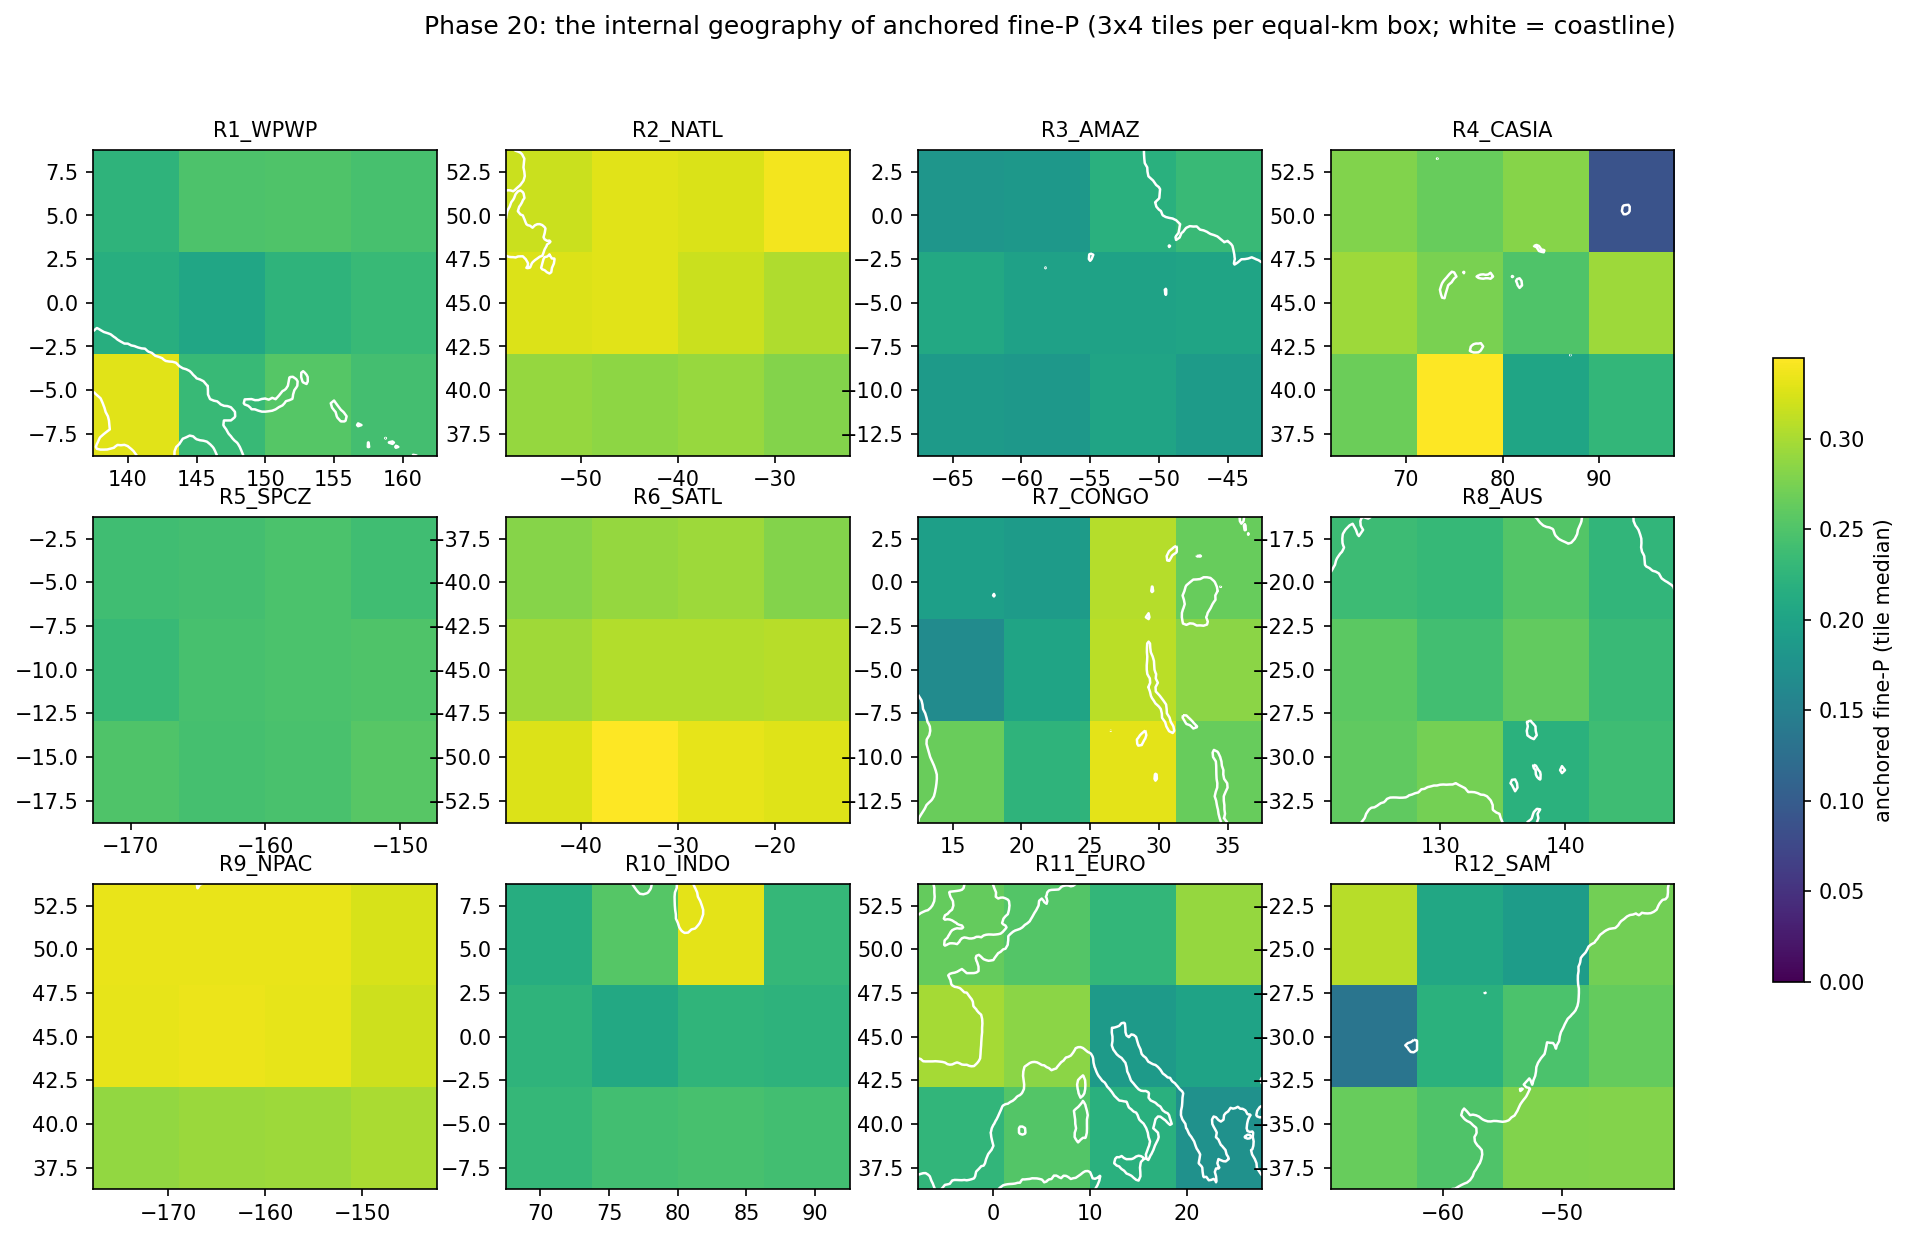
\includegraphics[width=\linewidth]{figures/fig2_tile_maps.png}
\caption{Внутренняя география тонкомасштабного $P$ с суррогатной поправкой (полосы 50--400~км): 12 равновеликих областей $\times$ 12 тайлов, медианы по окнам; белым --- береговая линия. Максимумы приходятся на области внетропических штормовых путей --- североатлантическую (R2), южноатлантическую (R6) и северотихоокеанскую (R9); минимумы --- на ядра глубокой конвекции (запад бассейна Конго, Амазония) и на северо-восточный тайл Центральной Азии.}
\label{fig:tiles}
\end{figure}

\begin{figure}[t]
\centering
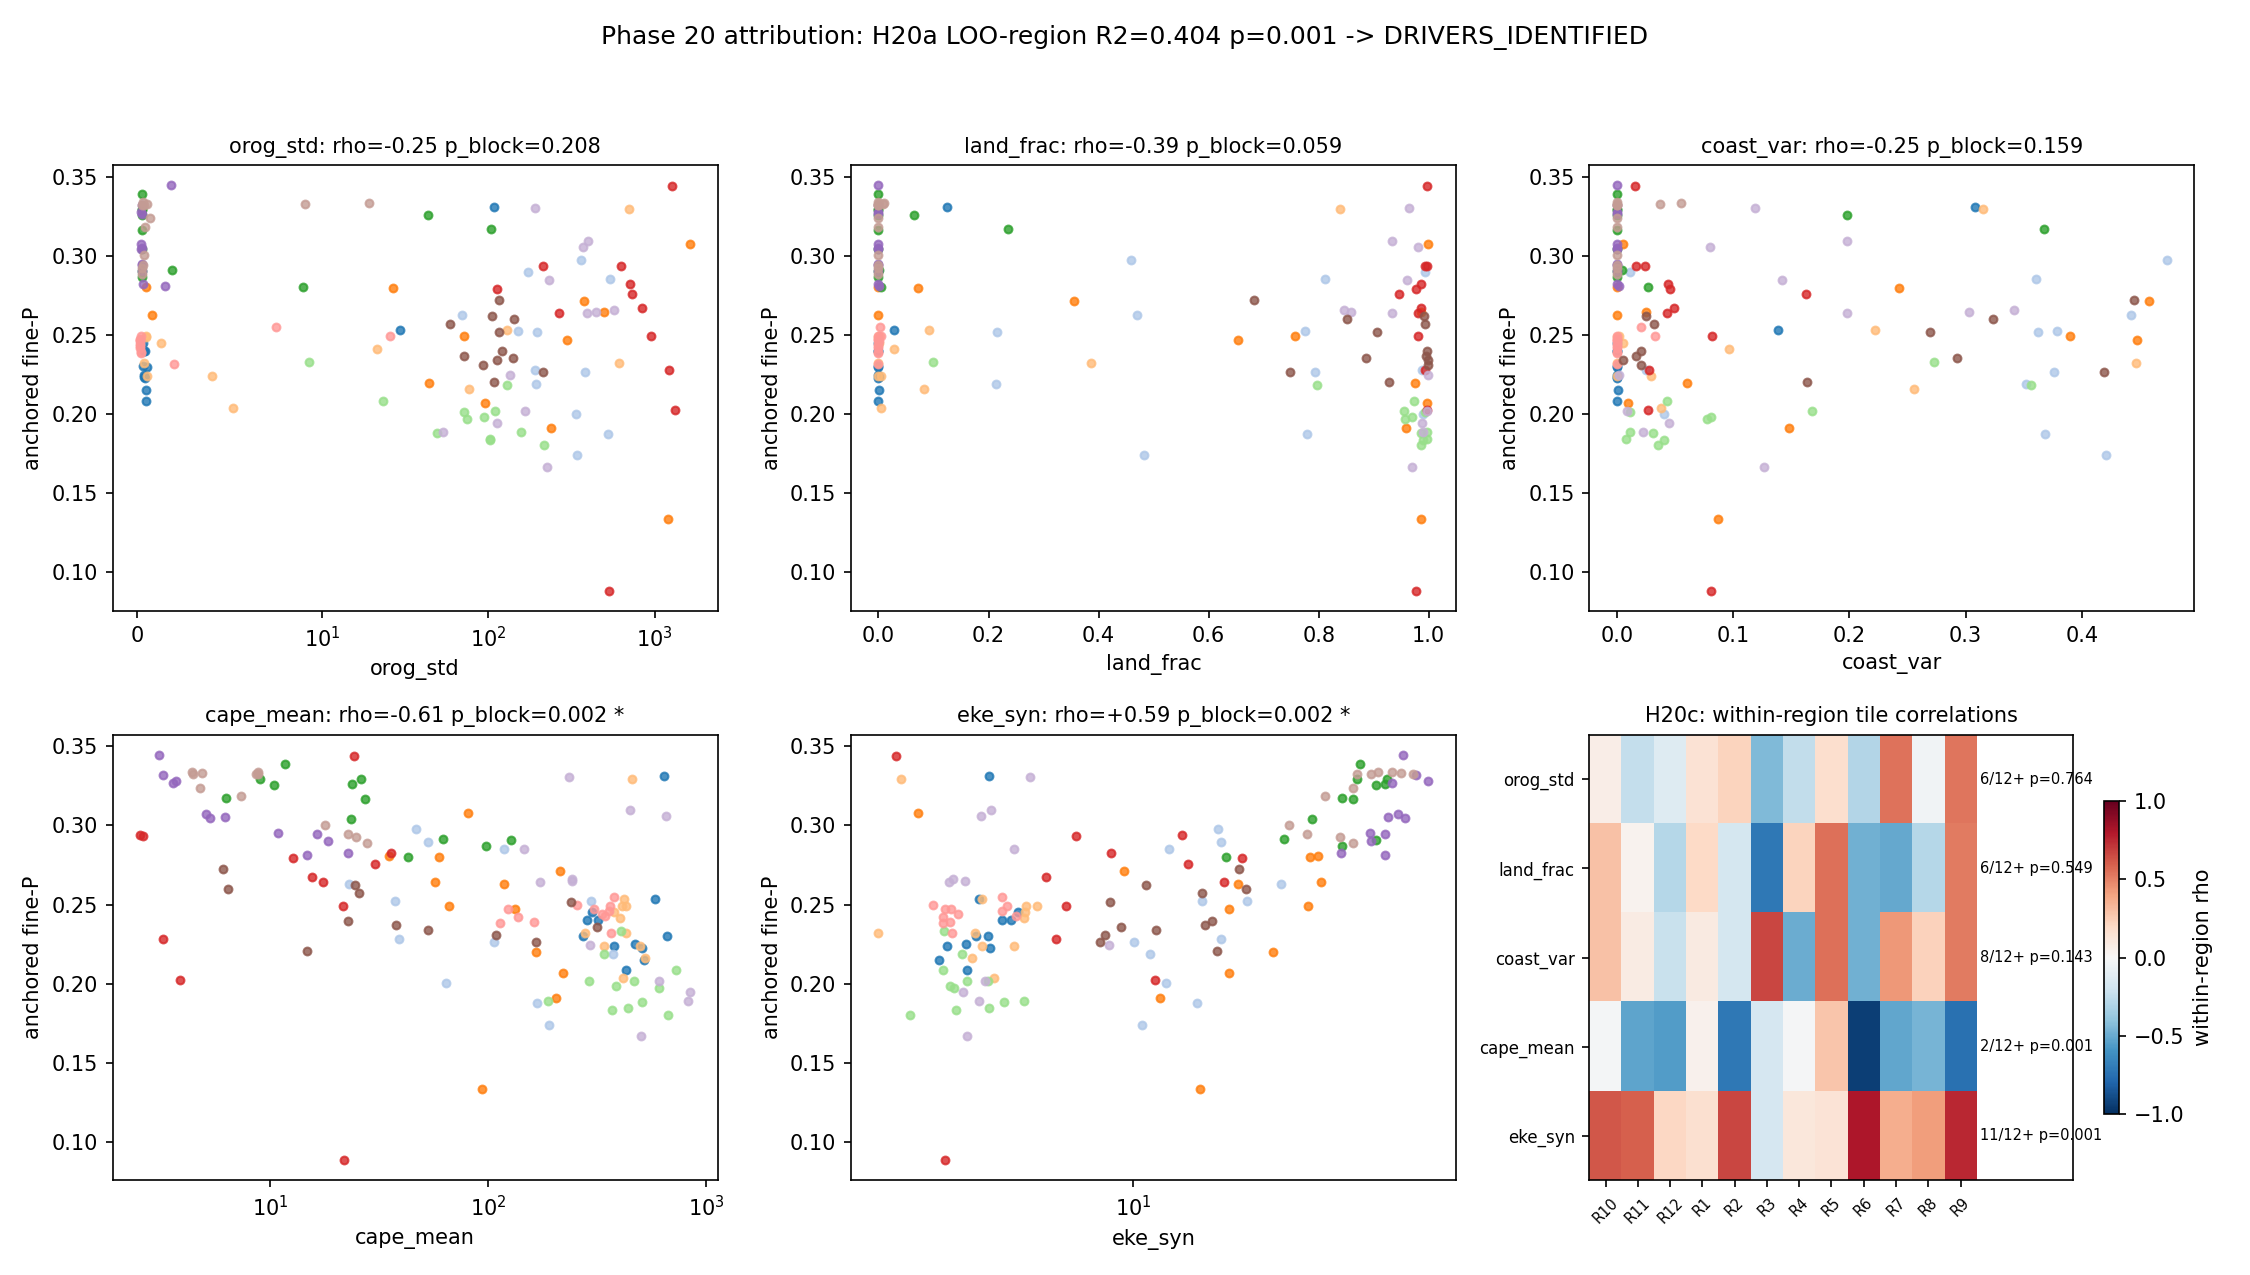
\includegraphics[width=\linewidth]{figures/fig2_attribution.png}
\caption{Часть A, атрибуция тайлового $P$: диаграммы рассеяния по пяти ковариатам с $p$-значениями блочного нуля (цвет --- регион; звёздочкой отмечены значимые связи) и тепловая карта внутрирегиональных корреляций (справа внизу): CAPE отрицательна в 10 из 12 регионов, синоптическая вихревая энергия положительна в 11 из 12.}
\label{fig:attrA}
\end{figure}

\subsection{Глобальная атрибуция: незональность, одна ось, два яруса (часть B)}
\label{sec:armB}

Атрибуция глобальной карты выполнена по восьми заранее заявленным ковариатам с выбыванием целых секторов долготы и нуль-моделью вращения; сводка --- в табл.~\ref{tab:armB}. Карта части~B согласована с картой части~A на 133 общих тайлах ($\rho=0{,}840$). Результат складывается в три утверждения.

\emph{Атрибуция значима, и её значимость незональна.} Восемь ковариат предсказывают карту вне сектора подгонки с $R^2=0{,}536$ ($p=0{,}001$ при 95-м перцентиле нуля 0,455). Поскольку нуль-модель вращения сохраняет всю зональную структуру целиком, значимость удостоверяет привязку карты к \emph{конкретному долготному положению} штормовых путей и конвективных очагов; ни широтный ход разд.~\ref{sec:geo}, ни контраст суши и океана сами по себе такого результата дать не могут. Отрицательный контроль чист: индекс листовой поверхности даёт прирост $-0{,}004$ ($p=0{,}832$).

\emph{Карта эффективно одномерна.} Пошаговый отбор показывает, что одна ковариата --- вихревая энергия --- даёт $R^2=0{,}456$, то есть 85\,\% полного качества предсказания ($k_{80}=1$). География сопряжённости, взятая как задача районирования, упорядочивается практически одной осью, и эта ось --- активность внетропических штормовых путей. Это статистическое выражение того, что видно на карте: кольцо Южного океана и северные штормовые пути --- её главный рисунок.

\emph{Оба яруса читают одну карту.} Один ярус~1 (экзогенные граничные условия) даёт $R^2=0{,}482$ при $p=0{,}002$, а ярус~2 добавляет к этому лишь $+0{,}053$: 90\,\% полного качества предсказания восстанавливается по одним лишь стационарным условиям территории --- широте, градиенту ТПО, подстилающей поверхности. Одновременно наибольшую индивидуальную нагрузку несёт характеристика яруса~2, и её связь с~$P$ сохраняется внутри регионов (разд.~\ref{sec:armA}). Противоречия нет: климатическое положение штормовых путей и очагов глубокой конвекции само есть следствие распределения материков, океанов и горных систем, поэтому два яруса читают одну и ту же карту с разных сторон. Следствия для выбора между H1 и H2 разобраны в разд.~\ref{sec:interp}.

\begin{table}[t]
\centering
\caption{Часть B: сводка проверок на глобальной сетке (902 тайла после орографического исключения). LOSO --- выбывание по сектору долготы $60^\circ$; нуль --- вращение долготной сетки ковариат (999 повторов).}
\label{tab:armB}
\small
\begin{tabular}{@{}p{0.46\linewidth}p{0.48\linewidth}@{}}
\toprule
Проверка & Итог\\
\midrule
Согласованность с частью A (133 общих тайла) & $\rho=0{,}840$ (заранее заданный порог 0,7)\\
Атрибуция, выбывание по сектору & $R^2=0{,}536$; $p=0{,}001$ (95-й перцентиль нуля 0,455)\\
Разделение по ярусам & ярус 1 (граничные условия): $R^2=0{,}482$ ($p=0{,}002$); прирост от яруса 2: $+0{,}053$\\
Эффективная размерность & одна вихревая энергия: $R^2=0{,}456$, т.\,е. 85\,\% полного качества; $k_{80}=1$\\
Потолок надёжности карты (внутрисезонное расщепление пополам) & $R^2=0{,}914$; атрибуция объясняет 59\,\% воспроизводимой дисперсии\\
Контрольная мишень: наклон спектра & $R^2=0{,}570$ --- не хуже целевой величины, но с непересекающимся набором ведущих ковариат (рельеф и доля суши вместо вихревой энергии, широты, градиента ТПО и CAPE)\\
Отрицательный контроль (индекс листовой поверхности) & прирост $-0{,}004$; $p=0{,}832$ --- контроль чист\\
Сезонная устойчивость карты & медиана $\lvert$ЯФМ$-$ИАС$\rvert=0{,}016$ (ЯФМ --- январь--март, ИАС --- июль--сентябрь), 90-й перцентиль 0,048\\
\bottomrule
\end{tabular}
\end{table}

\subsection{Два канала: через спектр и сверх спектра}
\label{sec:channels}

Главный содержательный результат атрибуции виден не в величине $R^2$, а в составе нагрузок (табл.~\ref{tab:loadings}, рис.~\ref{fig:channels}). Контрольная мишень --- наклон пространственного спектра тайла --- предсказывается теми же восемью ковариатами \emph{не хуже} целевой величины ($R^2=0{,}570$ против $0{,}536$), но наборы ведущих ковариат у двух мишеней практически не пересекаются: сопряжённость нагружают вихревая энергия ($+0{,}66$), модуль широты ($+0{,}66$), градиент ТПО ($+0{,}55$) и CAPE ($-0{,}52$), а спектральный наклон --- расчленённость рельефа ($+0{,}74$), доля суши ($+0{,}67$), средняя высота рельефа ($+0{,}65$) и изрезанность берега ($+0{,}63$); ведущие ковариаты одной мишени лежат в полосе $\lvert\rho\rvert<0{,}3$ у другой. Это отвечает на вопрос, оставленный открытым в разд.~\ref{sec:geo}: контраст суши и океана в карте~$P$ --- не контраст подстилающей поверхности как таковой (её читает спектр), а контраст режимов.

Описательное двухслойное прочтение части~A (апостериорное, помеченное так и в протоколе) уточняет структуру связи. Если перед атрибуцией удалить из тайлового~$P$ часть, линейно предсказуемую по спектральным признакам самого тайла, совместная атрибуция исчезает ($R^2=-0{,}055$, $p=0{,}15$), однако отрицательная связь с CAPE выживает внутри регионов (10 из 12, средняя $\rho=-0{,}34$), а связь с вихревой энергией --- нет (8 из 12, $\rho\approx+0{,}03$). Отсюда двухканальная \emph{структура связи}: повышение сопряжённости при высокой штормовой активности идёт через ту же дисперсионную структуру, которую видит спектр, а понижение при высокой конвективной неустойчивости лежит сверх спектра. Правдоподобное, но не проверенное здесь прочтение: интермиттентная завихренность мезомасштабных конвективных систем \cite{Houze2004,Feng2021,PetersNeelin2006}, порождающая собственную изменчивость, слабо связанную с крупным масштабом \cite{Zhang2007,RotunnoSnyder2008,Judt2020}, ослабляет со-организацию уровней, а организованные бароклинные возмущения штормовых путей её усиливают. Установлены связь и её канальное разделение, но не механизм.

\begin{table}[t]
\centering
\caption{Нагрузки восьми ковариат (ранговая корреляция по 902 тайлам) на две мишени: $P$ с суррогатной поправкой и наклон пространственного спектра тайла. Мишени предсказываются сопоставимо хорошо ($R^2_{\mathrm{LOSO}}=0{,}536$ и $0{,}570$), но ведущими для них оказываются непересекающиеся наборы ковариат. Ярус~2 отмечен звёздочкой.}
\label{tab:loadings}
\small
\begin{tabular}{@{}lcc@{}}
\toprule
Ковариата & $P$ с поправкой & Наклон спектра\\
\midrule
Синоптическая вихревая энергия${}^{*}$ & $+0{,}66$ & $-0{,}12$\\
Модуль широты & $+0{,}66$ & $-0{,}05$\\
Градиент ТПО & $+0{,}55$ & $-0{,}27$\\
Климатология CAPE${}^{*}$ & $-0{,}52$ & $+0{,}22$\\
Доля суши & $-0{,}17$ & $+0{,}67$\\
Орография (станд. отклонение) & $-0{,}14$ & $+0{,}74$\\
Орография (средняя высота) & $-0{,}11$ & $+0{,}65$\\
Контрастность суша--море & $-0{,}05$ & $+0{,}63$\\
\bottomrule
\end{tabular}
\end{table}

\begin{figure}[t]
\centering
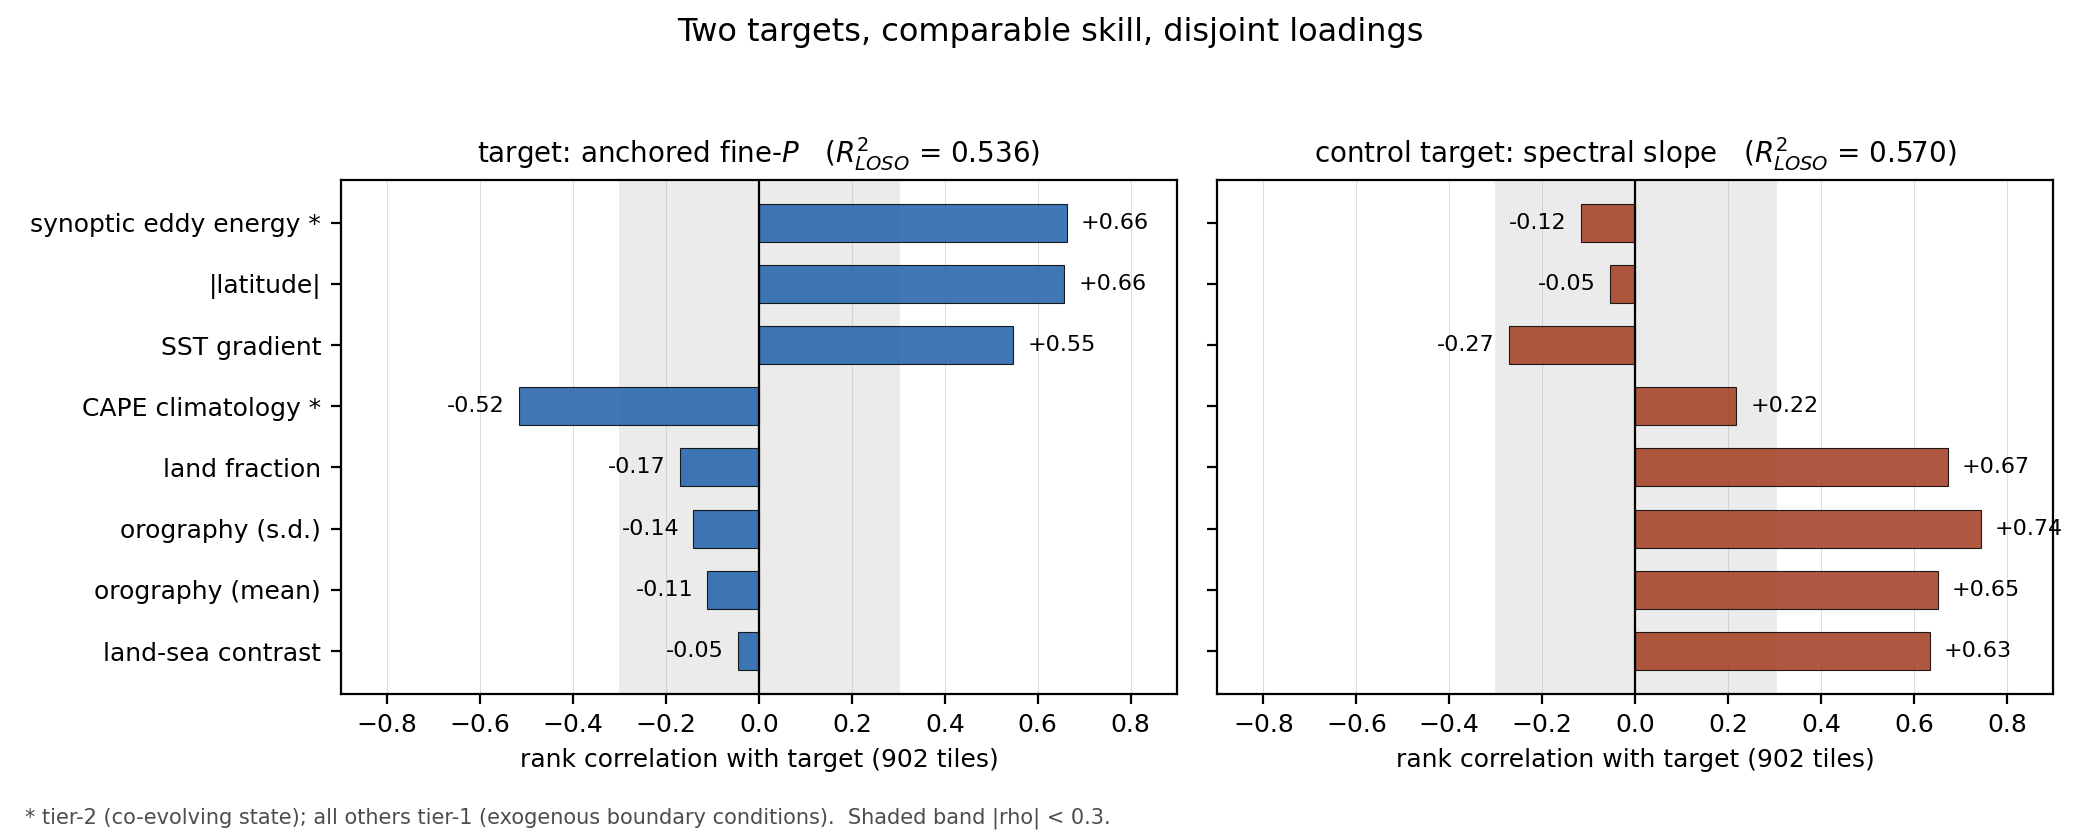
\includegraphics[width=\linewidth]{figures/fig2_channels.png}
\caption{Двухканальная структура связи: нагрузки восьми ковариат на две мишени глобальной тайловой карты --- $P$ с суррогатной поправкой (слева) и наклон пространственного спектра (справа), 902 тайла. Серая полоса отмечает диапазон $\lvert\rho\rvert<0{,}3$; ведущие ковариаты каждой мишени попадают внутрь этой полосы у другой. Звёздочкой помечены характеристики яруса~2, остальные --- ярус~1.}
\label{fig:channels}
\end{figure}

\subsection{Полнота атрибуции и география остатка}
\label{sec:residual}

Долю карты, которую ковариаты объясняют, следует считать не от полной дисперсии, а от воспроизводимой её части. Потолок восстановимости карты, оценённый внутрисезонным расщеплением выборки пополам, составляет $R^2=0{,}914$; межсезонная оценка ($0{,}603$) занижает его, списывая реальное сезонное изменение карты на шум. Относительно этого потолка заявленные ковариаты объясняют 59\,\% воспроизводимой дисперсии: карта атрибутирована, но далека от насыщения. Добавление блока из четырёх статистик интермиттентности огибающих --- ближайших родственников~$P$, восходящих к уточнённой гипотезе подобия \cite{Kolmogorov1962}, --- поднимает совместную модель до $R^2=0{,}761$, то есть до 83\,\%; прирост сохраняется при вычислении~$P$ и статистик интермиттентности на непересекающихся половинах выборки ($+0{,}207$, $p=0{,}001$).

Остаток после ковариат и блока интермиттентности --- около 15\,\% воспроизводимой дисперсии --- \emph{не является шумом}. Он воспроизводится между независимыми половинами выборки ($r=0{,}64$ при пороге решающего правила $0{,}30$), не сводится к спектральным признакам ($\lvert\rho\rvert\le0{,}12$ с наклоном и логарифмическими дисперсиями полос) и обнаруживает географически организованный рисунок (рис.~\ref{fig:residual}). Отрицательные значения --- сопряжённость ниже предсказанной по условиям --- образуют два субтропических пояса (средний остаток $-0{,}011$ на $30$--$40^\circ$ обоих полушарий) и сгущаются на муссонных окраинах и в предгорьях: Южный Китай, Средиземноморье и Анатолия, Иранское нагорье, побережье Красного моря, окраина Мексиканского нагорья, Андское предгорье и Патагония \cite{RodwellHoskins1996}. Положительные --- сопряжённость выше предсказанной --- лежат над очагами глубокой конвекции (северо-запад Амазонии, Конго, Эфиопское предгорье, Новая Гвинея, Гангская равнина) и над высокоширотными окраинами материков ($+0{,}015$ на $50$--$60^\circ$~с.\,ш.: Лабрадор, Гудзонов залив, север Евразии), а также в секторе Южного океана. Остаток лишь отчасти сезонно устойчив (ранговая согласованность двух сезонов 0,41): часть его рисунка меняется вместе с муссонами.

Попытка атрибутировать остаток предпринята по отдельному, зафиксированному до вычислений протоколу и завершилась отрицательным вердиктом; её изложение отнесено в разд.~\ref{sec:limitations}, чтобы не смешивать установленный факт существования остатка с неудавшимся объяснением.

\begin{figure}[t]
\centering
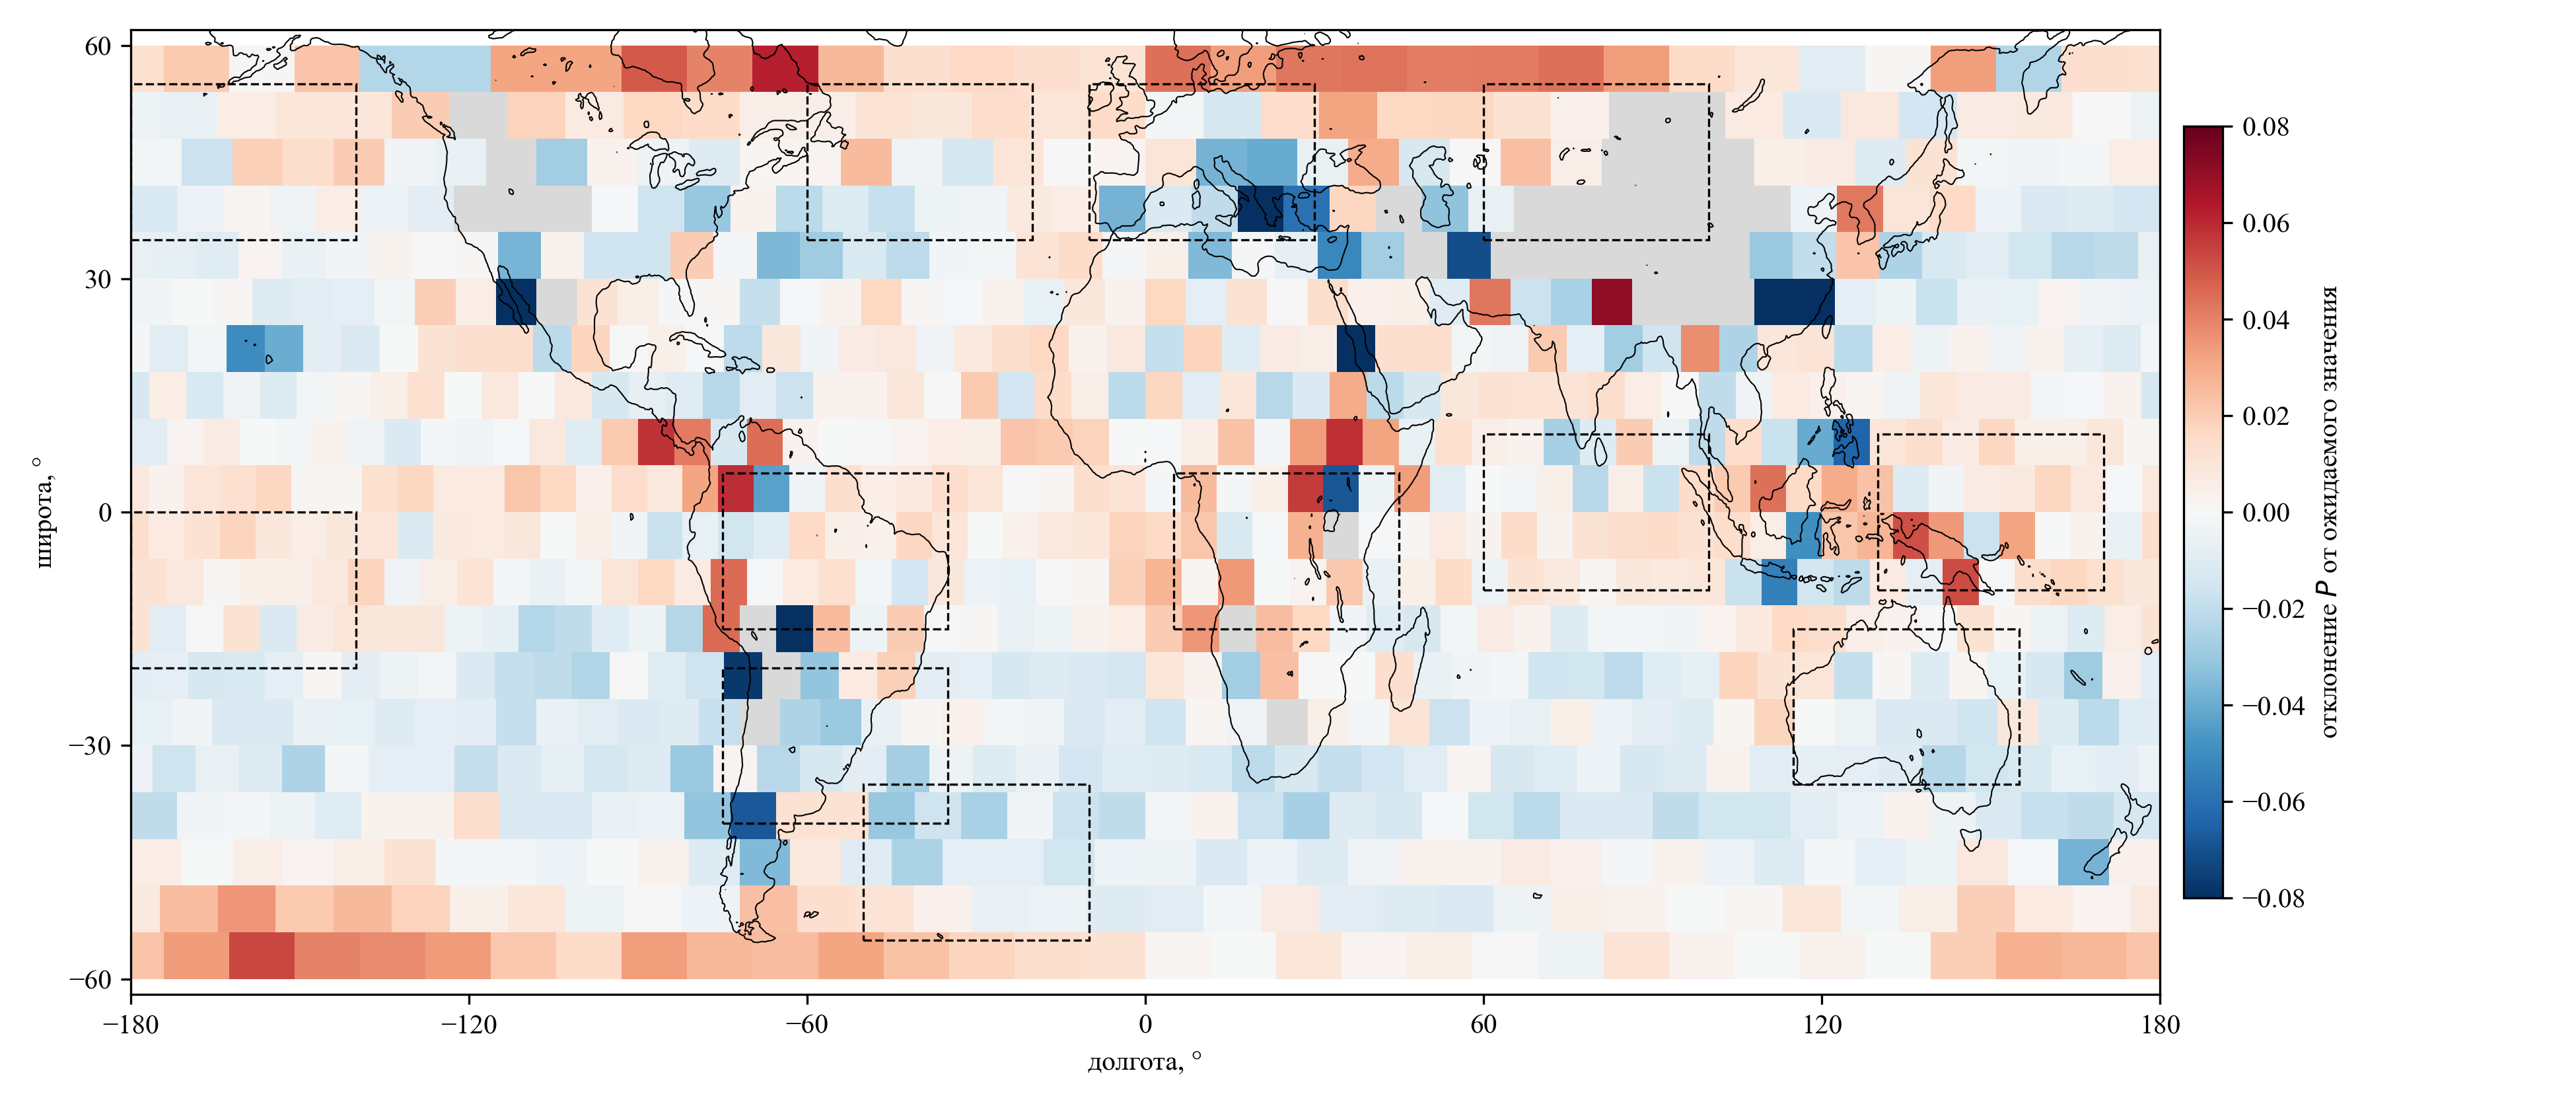
\includegraphics[width=\linewidth]{figures/fig2_residual_map.png}
\caption{Остаток глобальной карты $P$ после восьми ковариат атрибуции и блока статистик интермиттентности (среднее двух сезонов 2023~г.; регрессия обучена на противоположной временной половине выборки, поэтому остаток свободен от общего выборочного шума). Синим --- сопряжённость ниже предсказанной (субтропические муссонные окраины, предгорья), красным --- выше (очаги глубокой конвекции, высокоширотные окраины материков). Серым --- тайлы, исключённые по орографии; штриховые рамки --- двенадцать областей программы.}
\label{fig:residual}
\end{figure}

\section{Природа карты: физика атмосферы или артефакт наблюдений}
\label{sec:model}

Сопоставление двух реанализов не отделяет свойство атмосферы от свойства наблюдательной сети: обе системы усваивают в основном одни и те же наблюдения \cite{Hersbach2020,Gelaro2017}; решающая проверка --- расчёт, не усваивающий наблюдений. Использован эксперимент \texttt{highresSST-present} проекта HighResMIP \cite{Haarsma2016} по модели ECMWF-IFS-HR \cite{Roberts2018}: расчёт типа AMIP --- атмосфера при заданной наблюдаемой температуре поверхности океана \cite{Gates1992}; глобальные поля 2014~г., разрешение $0{,}5^\circ$, без усвоения атмосферных наблюдений.

На 902 тайлах, согласованных по разрешению, ранговая корреляция эталонной пары <<ERA5 при $0{,}25^\circ$ --- ERA5 при $0{,}5^\circ$>> (одна и та же атмосфера, цена огрубления) составляет $0{,}897$ --- разрешающий предел сопоставления. Карта свободного расчёта воспроизводит карту ERA5 с $\rho=0{,}869$, то есть \emph{97\,\% достижимого согласия} (отношение ранговых корреляций, а не доля объяснённой дисперсии), при том что расчёт относится к 2014~г. против 2023~г. и не видел ни одного атмосферного наблюдения (рис.~\ref{fig:round2}, слева). Нагрузки на модельную карту повторяют реанализные: вихревая энергия $+0{,}68$, модуль широты $+0{,}70$, градиент ТПО $+0{,}51$, CAPE $-0{,}50$, рельеф $\approx0$. Недостающие три процента разрешающего предела --- того же порядка, что цена самого огрубления, и заведомо меньше различия двух лет и двух вычислительных трактов. Заранее зафиксированные условия признания ($\rho_{\mathrm{mod}}\ge0{,}5$ и $\rho_{\mathrm{mod}}\ge0{,}6\,\rho_{\mathrm{lim}}$) выполнены с запасом; H3 отвергается. (Пара $\rho=0{,}71$ при пределе $0{,}93$ из первой статьи относится к \emph{региональной} выборке по 39 областям и с приведённой здесь глобальной парой не взаимозаменяема.)

\begin{figure}[t]
\centering
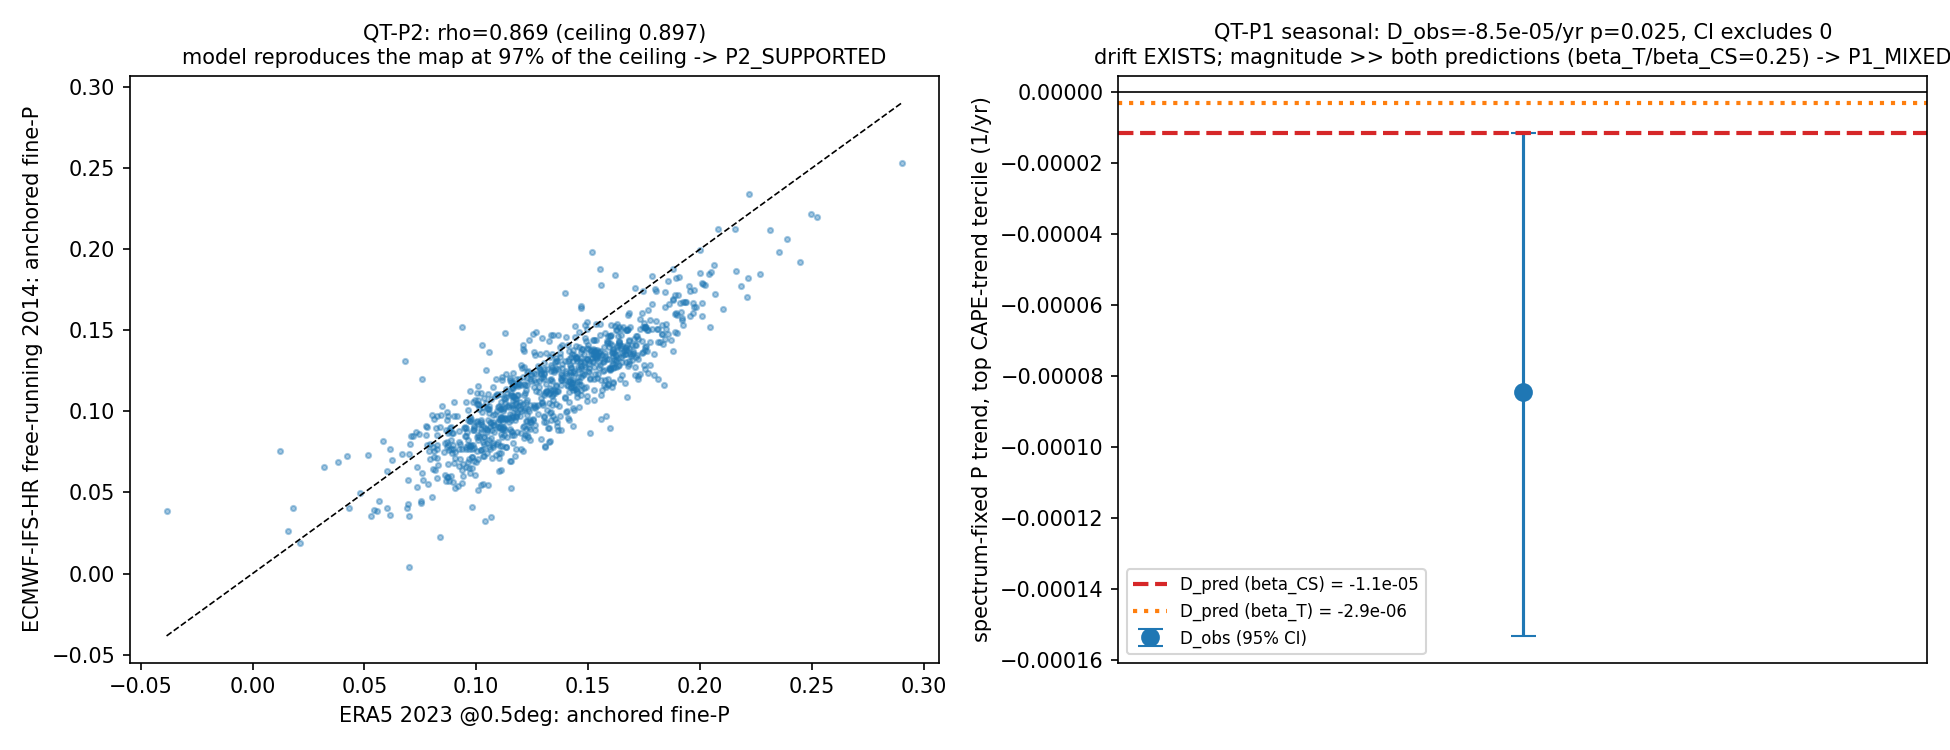
\includegraphics[width=\linewidth]{figures/fig2_qt_round2.png}
\caption{Слева: тайловая карта $P$ (с суррогатной поправкой) свободного расчёта ECMWF-IFS-HR (2014~г., без усвоения наблюдений) против карты ERA5 (2023~г.) на 902 согласованных по разрешению тайлах: $\rho=0{,}869$ при разрешающем пределе $0{,}897$; пунктир --- линия равенства. Справа: тренд спектрально-фиксированного $P$ в тайлах верхней терцили тренда CAPE (точка --- оценка, отрезок --- 95-\%-й доверительный интервал кластерного бутстрэпа) в сравнении с двумя калибровочными предсказаниями (штриховые линии); к разд.~\ref{sec:time}.}
\label{fig:round2}
\end{figure}

\section{Районирование по сопряжённости}
\label{sec:region}

Из установленного вытекает возможность районирования: карта~$P$ предсказуема по условиям, воспроизводится свободным расчётом, сезонно устойчива и несёт информацию, не сводимую к спектру, --- то есть удовлетворяет требованиям к координате районирования. Ниже предложена типология тайлов по двум осям --- организатору циркуляции и уровню сопряжённости (разд.~\ref{sec:data}); она описательна и служит не заменой атрибуции, а её географическим прочтением.

\begin{table}[t]
\centering
\caption{Типология 902 тайлов по организатору циркуляции (строки; глобальные терцили вихревой энергии и климатологии CAPE) и уровню сопряжённости (столбцы; терцили двухсезонного среднего $P$): число тайлов, среднее $P$ и доля океанических тайлов.}
\label{tab:typology}
\small
\begin{tabular}{@{}lccc@{}}
\toprule
Организатор & $P$ высокая ($\ge0{,}273$) & $P$ средняя & $P$ низкая ($\le0{,}244$)\\
\midrule
Штормовой путь (294 тайла) & \textbf{229}; 0,312; океан 90\,\% & 56; 0,264; 80\,\% & 9; 0,217; 11\,\%\\
Без ведущего организатора (312) & 38; 0,298; 50\,\% & \textbf{139}; 0,256; 86\,\% & 135; 0,227; 65\,\%\\
Конвективный режим (296) & 34; 0,307; 68\,\% & 105; 0,256; 86\,\% & \textbf{157}; 0,219; 66\,\%\\
\bottomrule
\end{tabular}
\end{table}

Таблица~\ref{tab:typology} и рис.~\ref{fig:region} показывают, что типология почти диагональна. Из 294 тайлов штормовых путей 229 (78\,\%) лежат в верхней терцили сопряжённости; из 296 конвективных 157 (53\,\%) --- в нижней; тайлы без ведущего организатора распределены между средней и нижней терцилями. Диагональные классы и есть главные провинции карты: \emph{штормовые пояса высокой сопряжённости} --- кольцо Южного океана, северные океанические штормовые пути и их высокоширотные материковые окраины; \emph{конвективные провинции низкой сопряжённости} --- экваториальные очаги Амазонии, Конго и Индонезийского архипелага и субтропические муссонные земли Южной и Восточной Азии, Аравии, Мексики; \emph{промежуточная провинция} --- субтропические океаны и внутриматериковые области умеренного пояса.

Не менее содержательны внедиагональные классы: это территории, где сопряжённость \emph{не} следует организатору, --- то есть география остатка разд.~\ref{sec:residual}, увиденная на языке типологии. Девять штормовых тайлов низкой сопряжённости почти все материковые (океан 11\,\%) и лежат на материковых окраинах южных штормовых путей --- Пампа и Патагония, юг Австралии: там, где путь выходит на сушу и на подветренную сторону Анд. Тридцать четыре конвективных тайла высокой сопряжённости --- преимущественно океанические и прибрежные (океан 68\,\%): акватория к югу от Явы, тихоокеанское побережье Центральной Америки и Колумбии, Новая Гвинея, Бенгальский залив и Гангская равнина --- области, где конвекция организована крупномасштабным потоком (пассатами, муссонным течением, береговыми линиями), а не свободной внутриматериковой неустойчивостью. Тридцать восемь тайлов высокой сопряжённости без ведущего организатора распадаются на два типа: восточно-пограничные побережья океанов с апвеллингом и сильными градиентами температуры поверхности (Калифорния, центральное Чили, Канарское и Португальское, Западная Австралия) и высокоширотная внутренняя Евразия ($51$--$57^\circ$~с.\,ш.); треть тайлов класса граничит с орографическим исключением --- единственный класс, где такая доля велика.

Для двенадцати областей программы типология даёт сводку в табл.~\ref{tab:regions}: три штормовые области (Северная Пацифика, Северная и Южная Атлантика) целиком лежат в верхней терцили, конвективные (Амазония, Конго, Индонезия) --- на 73--83\,\% в нижней, а области смешанного режима (Европа, субтропики Южной Америки, Австралия) внутренне неоднородны --- их региональное среднее скрывает контраст между тайлами разных классов. Именно эта внутренняя неоднородность и составляет те 49\,\% дисперсии, что лежат ниже регионального уровня (разд.~\ref{sec:armA}).

\begin{table}[t]
\centering
\caption{Двенадцать областей программы в типологии: число тайлов глобальной сетки с центром внутри области, среднее и размах $P$, преобладающий организатор, доли тайлов верхней и нижней терцилей.}
\label{tab:regions}
\small
\begin{tabular}{@{}lcccccc@{}}
\toprule
Область & $n$ & $P$ & размах & организатор & верхняя & нижняя\\
\midrule
R9 Северная Пацифика & 13 & 0,311 & 0,28--0,34 & штормовой & 100\,\% & 0\\
R2 Северная Атлантика & 14 & 0,305 & 0,27--0,34 & штормовой & 93\,\% & 0\\
R6 Южная Атлантика & 14 & 0,303 & 0,27--0,34 & штормовой & 93\,\% & 0\\
R4 Центральная Азия & 5 & 0,271 & 0,24--0,29 & без ведущего & 60\,\% & 20\,\%\\
R12 Южная Америка, субтропики & 19 & 0,255 & 0,18--0,36 & штормовой & 21\,\% & 37\,\%\\
R1 Тёплый бассейн зап. Пацифики & 24 & 0,252 & 0,20--0,32 & конвективный & 21\,\% & 46\,\%\\
R5 Юж.-Тихоокеанская зона конвергенции & 20 & 0,245 & 0,23--0,26 & конвективный & 0 & 45\,\%\\
R8 Австралия & 23 & 0,245 & 0,21--0,28 & без ведущего & 13\,\% & 48\,\%\\
R11 Европа & 13 & 0,243 & 0,15--0,31 & без ведущего & 31\,\% & 46\,\%\\
R10 Индонезия & 28 & 0,231 & 0,19--0,28 & конвективный & 4\,\% & 79\,\%\\
R7 Бассейн Конго & 22 & 0,220 & 0,11--0,28 & конвективный & 9\,\% & 73\,\%\\
R3 Амазония & 24 & 0,217 & 0,11--0,36 & конвективный & 8\,\% & 83\,\%\\
\bottomrule
\end{tabular}
\end{table}

\begin{figure}[t]
\centering
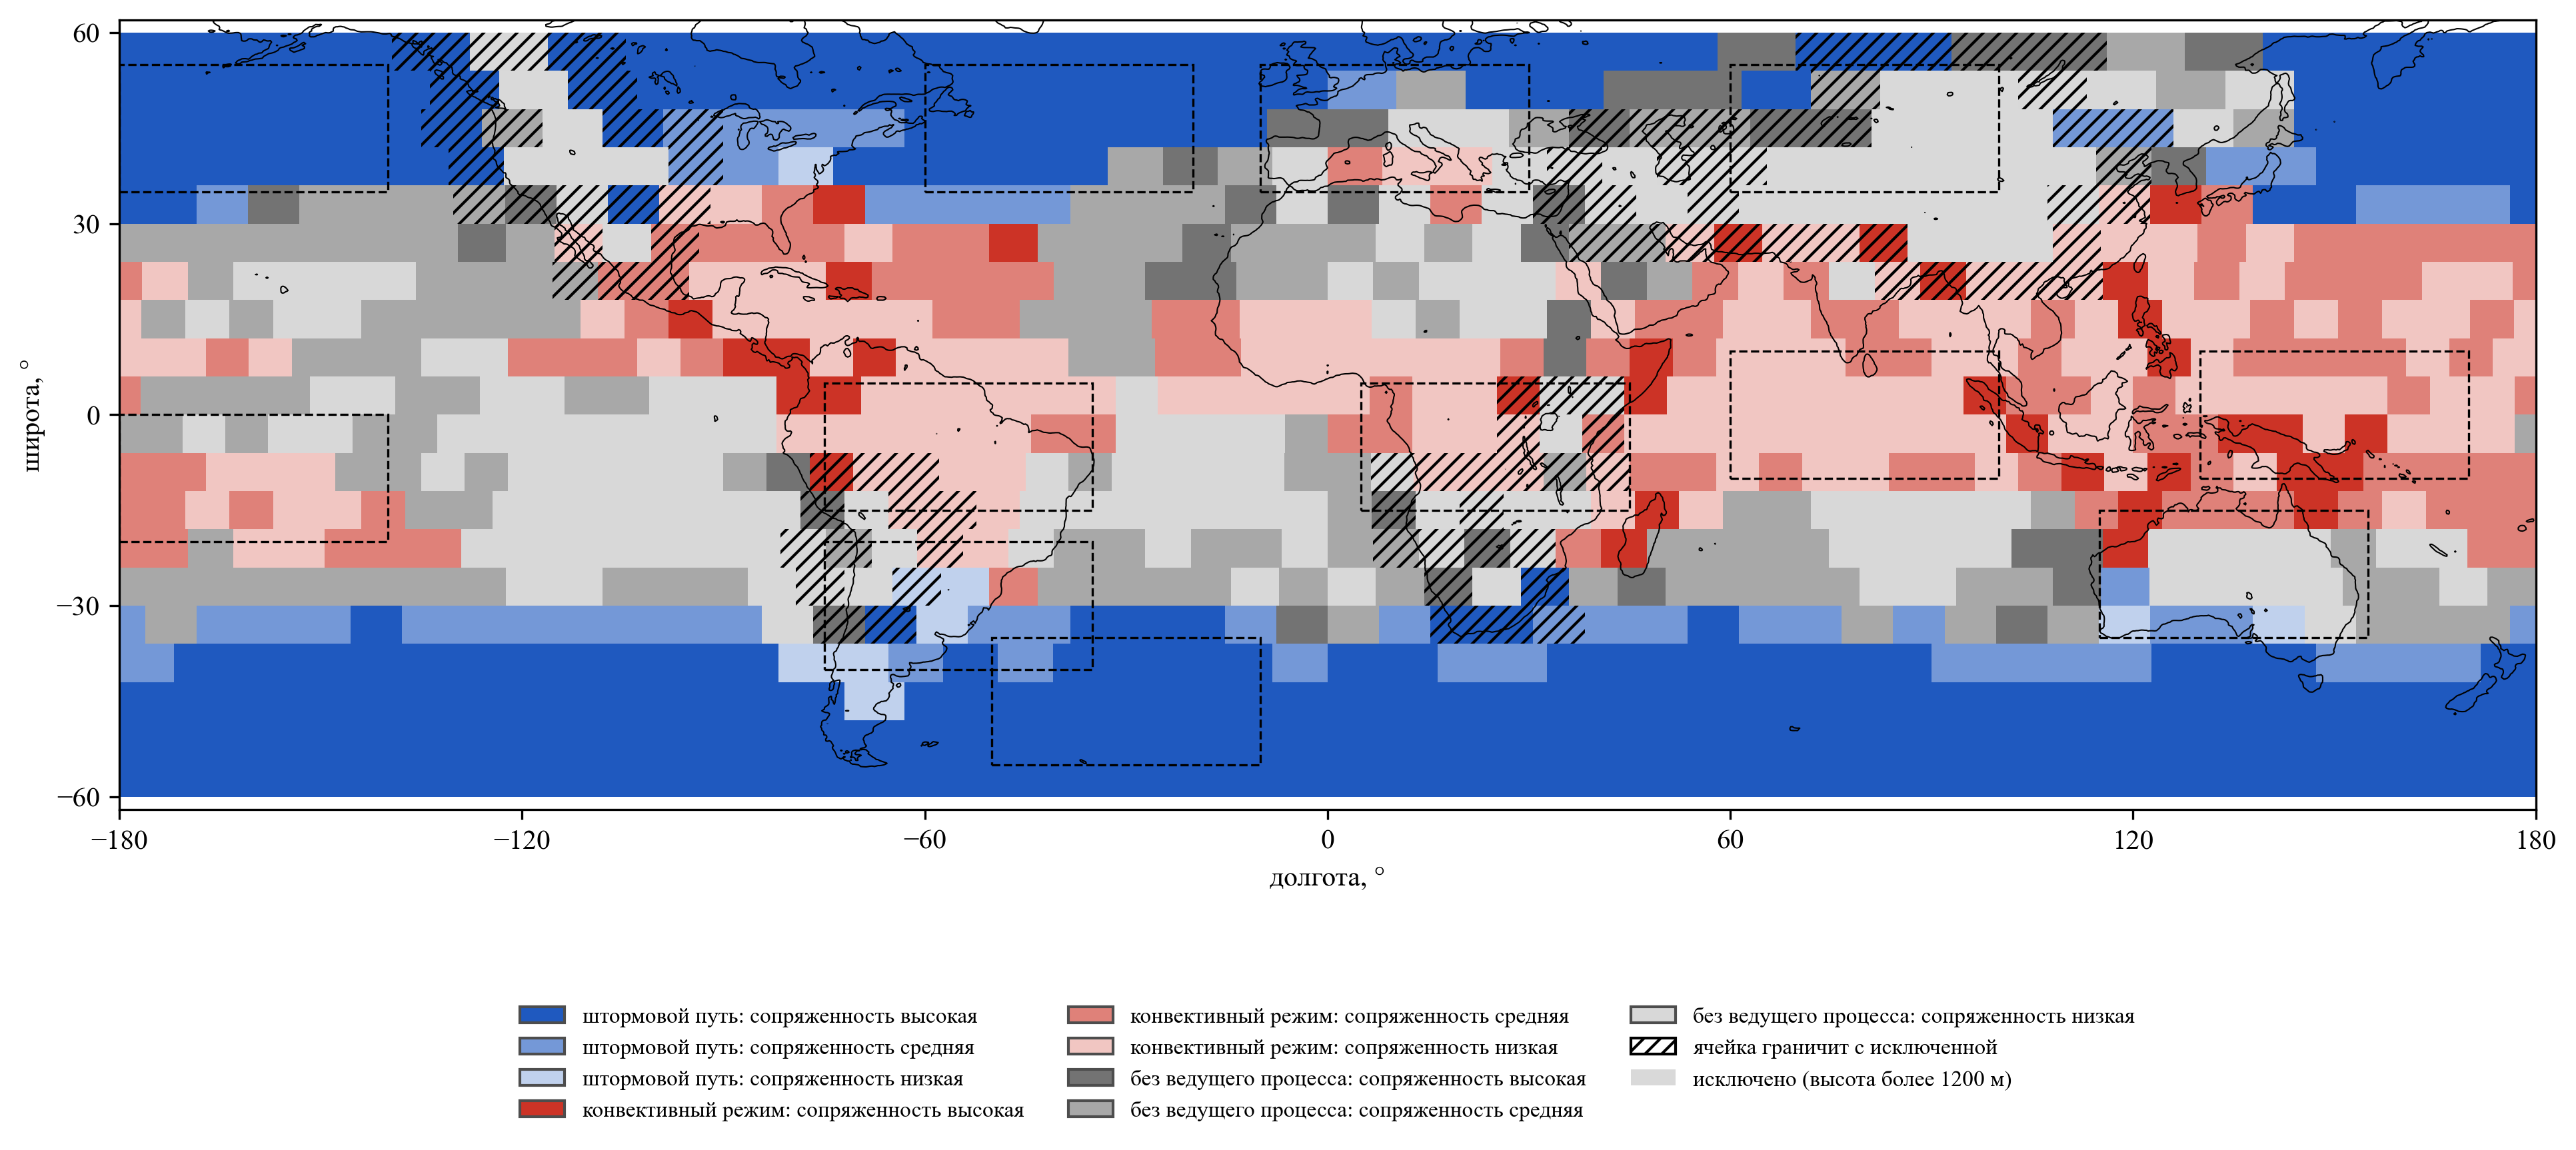
\includegraphics[width=\linewidth]{figures/fig2_regionalization.png}
\caption{Типология тайлов глобальной карты (описательно): цвет --- организатор циркуляции (синий --- штормовой путь, красный --- конвективный режим, серый --- без ведущего организатора), насыщенность --- терциль сопряжённости $P$ (тёмный --- высокая, светлый --- низкая). Штриховка --- тайлы, граничащие с исключёнными по орографии; светло-серым --- исключённые; штриховые рамки --- двенадцать областей программы.}
\label{fig:region}
\end{figure}

Два замечания о статусе типологии. Во-первых, границы терцилей --- условность, выбранная ради симметрии осей; районирование в строгом смысле потребовало бы обоснованных порогов и проверки устойчивости к ним, что здесь не делалось. Во-вторых, типология построена по одному году; её ценность --- в том, что она наглядно связывает три результата работы: одномерность атрибуции (диагональ), двухканальность (разные организаторы на разных концах оси) и географию остатка (внедиагональные классы).

\section{Время: тропический избыток и статичность}
\label{sec:time}

\emph{Тропический избыток межгодовой изменчивости.} На записи 1979--2024~гг. межгодовые значения инварианта в двенадцати областях программы устойчивы, за одним исключением: три очага глубокой конвекции --- тёплый бассейн запада тропической Пацифики, Амазония и Южно-Тихоокеанская зона конвергенции --- несут избыток межгодовой дисперсии ($F=1{,}75$; $2{,}24$; $2{,}07$ против $0{,}70$--$1{,}35$ у остальных), устойчивый к смене единицы выборки; связь с ЭНСО (индекс ONI \cite{Trenberth1997}) исключена прямым тестом при тридцатикратном превышении мощности относительно первоначальной проверки. Для атрибуции заранее назван список из четырёх индексов (PDO \cite{Newman2016}, AMO, DMI, IPO-TPI \cite{Henley2015}); статистика --- максимум ранговой корреляции по восьми комбинациям <<индекс $\times$ сглаживание>> с совместным нулём циклического сдвига, штрафующим за множественность (табл.~\ref{tab:ipo}, рис.~\ref{fig:ipo}). Совпадение ведущего индекса в двух регионах из трёх активирует заранее зафиксированное правило согласованности: избыток --- проявление \emph{декадной} моды, Междекадного тихоокеанского колебания (IPO) \cite{Power1999,Henley2015}, а не межгодового ЭНСО-режима; тёплый бассейн (самый слабый избыток) остаётся неатрибутированным.

\begin{table}[t]
\centering
\caption{Атрибуция тропического избытка межгодовой изменчивости по заранее названным индексам (максимум-статистика по 8 комбинациям <<индекс $\times$ сглаживание>>, совместный нуль циклического сдвига).}
\label{tab:ipo}
\small
\begin{tabular}{@{}lcccc@{}}
\toprule
Регион & $T=\max\lvert\rho\rvert$ & Лучший индекс & $p$ & Значимо\\
\midrule
Тёплый бассейн запада тропической Пацифики & 0,311 & PDO (5-летнее сглаж.) & 0,155 & нет\\
Амазония & 0,453 & IPO-TPI & 0,001 & да\\
Южно-Тихоокеанская зона конвергенции & 0,602 & IPO-TPI & 0,001 & да\\
\bottomrule
\end{tabular}
\end{table}

\begin{figure}[t]
\centering
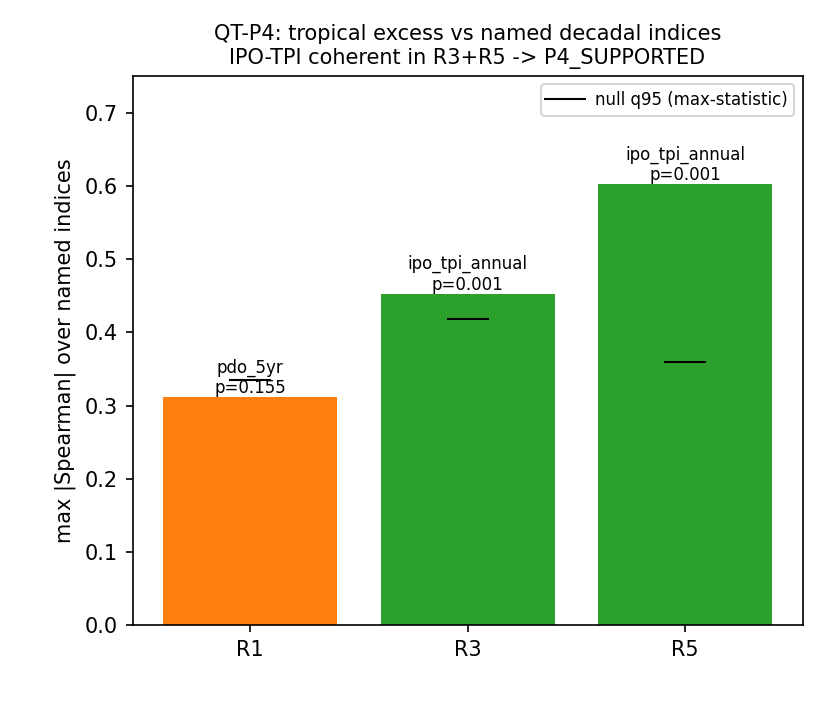
\includegraphics[width=0.6\linewidth]{figures/fig2_ipo.png}
\caption{Максимум-статистика связи межгодовой дисперсии карт активности с заранее названными климатическими индексами для трёх очагов тропического избытка межгодовой изменчивости; горизонтальные отрезки --- 95-е перцентили совместного нуля циклического сдвига. В Амазонии (R3) и Южно-Тихоокеанской зоне конвергенции (R5) значим один и тот же индекс --- IPO-TPI.}
\label{fig:ipo}
\end{figure}

\emph{Проверка гипотезы статичности.} Единственный крупный документированный сдвиг внутри записи --- переход IPO 1998/99~гг. На 72 парах <<тайл--сезон>> трёх тропических регионов~$P$ реагирует на переход раньше или резче конкурента реже порога опережающего поведения 60\,\% (25\,\% против CAPE, 47\,\% против вихревой энергии, 42\,\% против наклона спектра), а по медианному отношению <<сигнал/шум>> многолетнего тренда на 288 парах занимает последнее место из четырёх показателей (0,67 против 2,39 у CAPE, 1,03 у наклона спектра, 0,85 у вихревой энергии; гипотеза о превосходстве~$P$ отвергается во всех парных сравнениях). Для инварианта, не несущего собственной динамики, это ожидаемое поведение: величина регистрирует архитектуру сложившегося режима, а не предвещает его перестройку.

\emph{Открытым остаётся вопрос о многодесятилетней устойчивости самих условий.} В тайлах верхней терцили тренда CAPE обнаружен слабый отрицательный тренд спектрально-фиксированного~$P$ ($-8{,}5\cdot10^{-5}$~год$^{-1}$, $p=0{,}025$, интервал кластерного бутстрэпа исключает ноль; рис.~\ref{fig:round2}, справа), в семь раз превышающий кросс-секционную калибровку по контрасту CAPE, тогда как единственный свободный расчёт с переходным форсингом воспроизводит его лишь на $\sim$27\,\% величины и неотличимо от нуля ($p=0{,}221$). Факт установлен только внутри ERA5 --- записи со сменами наблюдательной системы \cite{Bengtsson2004} --- и модельного подтверждения не имеет.

\section{Интерпретация, обсуждение и ограничения}
\label{sec:interp}

\subsection{Ответ на исходные гипотезы}

Соберём ответы (табл.~\ref{tab:hyp}). \emph{H3 отвергнута}: карта воспроизводится расчётом, не усваивающим атмосферных наблюдений, и потому не может быть артефактом наблюдательной сети. \emph{H1 и H2 обе подтверждены --- и именно это составляет результат.} Наибольшую индивидуальную нагрузку несёт характеристика яруса~2, и её связь с~$P$ сохраняется внутри регионов, где экзогенные условия почти постоянны; одновременно один ярус~1 восстанавливает 90\,\% полного качества предсказания. Данные при этом \emph{не} позволяют утверждать, будто рельеф и океан действуют исключительно опосредованно, через режимы: при 90\,\% качества у одного яруса~1 такое утверждение было бы сильнее данных.

\begin{table}[t]
\centering
\caption{Статус трёх гипотез и общих условий пригодности карты. Решающие правила зафиксированы протоколами до вычислений (разд.~\ref{sec:hypotheses}); там, где протокол числового порога не содержал, он не вводится задним числом.}
\label{tab:hyp}
\small
\begin{tabular}{@{}p{0.20\linewidth}p{0.15\linewidth}p{0.57\linewidth}@{}}
\toprule
Положение & Статус & Решающее правило и наблюдённое значение\\
\midrule
Пригодность карты & выполнено & порог $\rho\ge0{,}7$; наблюдено 0,874 (тайлы против региональных значений) и 0,840 (части A и B на 133 общих тайлах)\\
H1, экзогенная & подтверждена & числового порога не задавалось; ярус~1 отдельно даёт $R^2=0{,}482$ при $p=0{,}002$ --- 90\,\% полного качества предсказания\\
H2, циркуляционная & подтверждена & знак связи внутри регионов совпадает не менее чем в 10 регионах из 12; наблюдено 10/12 для CAPE (средняя $\rho=-0{,}36$) и 11/12 для вихревой энергии (средняя $\rho=+0{,}39$), в обоих случаях $p=0{,}001$\\
H3, артефактная & отвергнута & признание при $\rho_{\mathrm{mod}}\ge0{,}5$ и $\ge0{,}6\,\rho_{\mathrm{lim}}$; наблюдено $\rho_{\mathrm{mod}}=0{,}869$ при $\rho_{\mathrm{lim}}=0{,}897$, то есть $0{,}97\,\rho_{\mathrm{lim}}$\\
Эффективная размерность & выполнено & порог $k_{80}\le3$; наблюдено $k_{80}=1$\\
Отрицательный контроль & чист & значимый прирост означал бы смешение; наблюдено $-0{,}004$ при $p=0{,}832$\\
\bottomrule
\end{tabular}
\end{table}

Отсюда итоговая формулировка, объединяющая обе подтверждённые гипотезы и географическое описание: \emph{география сопряжённости уровней структурирована через размещение атмосферных циркуляционных режимов в географическом пространстве, а размещение самих режимов задано экзогенной конфигурацией территории}. Кольцо Южного океана высоко, потому что там штормовой путь не разорван материками; северные штормовые пути ниже и сезоннее, потому что разорваны; экваториальные и муссонные земли низки --- и понижаются во влажный сезон, --- потому что там организатором служит глубокая конвекция; побережья с сильными градиентами температуры поверхности образуют локальные максимумы, потому что там локализована бароклинность нижней тропосферы. Существенно, что речь идёт о географии, а не о широтной климатологии: около половины дисперсии карты лежит вне широтной составляющей, а нуль-модель вращения подтверждает, что атрибуция не сводится к широтному градиенту. В цепочке <<конфигурация $\to$ организация процессов $\to$ сопряжённость>> настоящей работой установлены оба крайних звена и их согласованность, но не механизм перехода между ними.

Разделение ковариат на ярусы задаёт и допустимый язык интерпретации. Для яруса~1 направленная формулировка <<граничные условия формируют географию сопряжённости>> корректна: эти поля экзогенны по отношению к циркуляции. Для яруса~2 направленный язык не используется: связь с~$P$ достигает максимума при нулевом временном сдвиге, без опережения в какую-либо сторону, и корректная формулировка --- \emph{совместное формирование}: сопряжённость, штормовая активность и конвективный режим суть согласованные проявления одной установившейся организации циркуляции. Профиль при этом естественно читать как наблюдаемую проекцию установившейся статистики быстрой динамики циркуляции при фиксированном на масштабе наблюдения поле внешних условий; развёртывание этой интерпретации --- предмет третьей статьи серии.

\subsection{Обсуждение и ограничения}
\label{sec:limitations}

Совокупность результатов складывается в определённый статус величины: география сопряжённости уровней --- не случайный рисунок и не артефакт наблюдательной системы, а физически атрибутируемая, эффективно одномерная и воспроизводимая карта, читаемая на языке известных организаторов циркуляции. Отдельно о весе двухканального результата: спектр поля скорости --- давно описанная и в общих чертах универсальная характеристика \cite{NastromGage1985,Lovejoy2011}, и его пространственная изменчивость управляется свойствами подстилающей поверхности. Если бы география~$P$ читалась тем же набором условий, величина была бы лишь иным способом измерить спектр. Наблюдается противоположное, и потому сопряжённость уровней может служить самостоятельной координатой районирования.

\emph{Остаток и попытки его атрибуции.} Источники воспроизводимого остатка (разд.~\ref{sec:residual}) не найдены. Орографический кандидат (расстояние до ближайшего рельефа выше 1200~м) прироста не даёт. Блок из четырёх гидроклиматических кандидатов --- годовая амплитуда осадков, конвективная доля осадков, вертикальный сдвиг ветра 850--500~гПа, влагозапас, --- проверенный по отдельному зафиксированному до вычислений протоколу, порога не проходит ($+0{,}024$ при пороге $+0{,}03$): три кандидата поглощены базовым набором через конвективно-влажностный канал. Единственная находка --- вертикальный сдвиг ветра: лишь он значимо связан с остатком ($\rho=-0{,}38$, $p=0{,}001$ при вращательном нуле), связь не опосредована спектром, знак (больше сдвиг --- сопряжённость ниже предсказанной) согласуется с географией отрицательного остатка на муссонных окраинах, а сам сдвиг --- классический управляющий параметр организации конвекции \cite{RotunnoKlempWeisman1988,Wing2017}. Вердикт тем не менее отрицательный, и утверждение об атрибуции остатка не делается.

Пять ограничений. Во-первых, полосы 50--400~км частично лежат ниже эффективного разрешения реанализа (разд.~\ref{sec:data}); величина определена операционально --- на выходе систем класса реанализа и глобальной модели ($0{,}25$--$0{,}5^\circ$), и её перенос на наблюдения километрового разрешения --- открытый вопрос. Во-вторых, глобальная карта и типология построены по одному году (2023); смягчают это сезонная устойчивость карты, согласованность с частью~A (окна 2021--2024~гг.) и воспроизведение карты расчётом 2014~г., но многолетняя глобальная карта остаётся задачей отдельной работы. В-третьих, природа карты проверена одним свободным расчётом одной модели; желательны ансамбль и модель с иным динамическим ядром. В-четвёртых, вихревая энергия вычисляется из того же поля ветра, что и профиль, и часть их связи может быть завышена общим источником; верхнюю границу инфляции даёт атрибуция по независимым полям яруса~1 ($R^2=0{,}482$ из $0{,}536$). В-пятых, многолетний тренд установлен только внутри ERA5 и не подтверждён свободным расчётом (разд.~\ref{sec:time}).

Наконец, о применении. Прогностическое содержание величины в первой статье проверялось и не подтвердилось; здесь этот вопрос не пересматривается. Но из установленного --- карта предсказуема по условиям, воспроизводится свободным расчётом на 97\,\% достижимого согласия и допускает типологию территорий --- следует по меньшей мере одно употребление: карта пригодна как \emph{диагностика воспроизведения мезомасштабной организации} в климатических моделях, поскольку задаёт наблюдаемую цель, не зависящую ни от усвоения наблюдений, ни от абсолютной амплитуды поля. Такая оценка остаётся предложением для дальнейших исследований.

\section{Выводы}
\label{sec:conclusion}

1.~\emph{Планетарная карта сопряжённости --- физико-географическая.} Её максимумы --- кольцо штормовых путей Южного океана (0,35--0,41) и северные океанические штормовые пути, минимумы --- экваториальные очаги глубокой конвекции и субтропические муссонные земли (0,10--0,18). Сопряжённость монотонно растёт от экватора (0,23) к умеренным широтам (0,32--0,35), над океаном выше, чем над сушей, во всех поясах, а в умеренных широтах Южного полушария выше, чем Северного, на 0,02--0,03 --- и при сравнении одних океанических тайлов. Половина дисперсии карты незональна.

2.~\emph{Сезонная география повторяет пространственную.} Карта сезонно устойчива (медиана контраста 0,016); её систематическая сезонность --- зимнее повышение в умеренных широтах Северного полушария и понижение в тропиках и субтропиках там и тогда, где активна муссонная конвекция.

3.~\emph{География карты атрибутируется, незональна и упорядочена одной осью.} Восемь внешних ковариат предсказывают карту вне подгонки на двух независимых выборках ($R^2=0{,}404$ при выбывании региона и $0{,}536$ при выбывании сектора долготы, $p=0{,}001$); нуль-модель вращения удостоверяет незональную часть; одна активность штормовых путей даёт 85\,\% полного качества ($k_{80}=1$). Половина географии сопряжённости лежит ниже регионального уровня, и мозаичная карта была условием такой проверки.

4.~\emph{Связь двухканальна.} Высокая штормовая активность сопровождается повышением сопряжённости через ту же дисперсионную структуру, которую отражает спектр; высокая конвективная неустойчивость --- её понижением сверх спектра. Контрольная мишень предсказывается теми же ковариатами не хуже, но непересекающимся их набором. Работа устанавливает атрибуцию, а не механизм.

5.~\emph{Экзогенная и циркуляционная гипотезы подтверждаются обе, артефактная отвергнута.} Стационарные условия территории сами по себе дают 90\,\% качества предсказания, тогда как наибольшую нагрузку несёт характеристика режима, сохраняющая связь внутри регионов; свободный расчёт без усвоения наблюдений воспроизводит карту с $\rho=0{,}869$ при пределе $0{,}897$. Итоговая формулировка: география сопряжённости структурирована через размещение циркуляционных режимов в географическом пространстве, а размещение режимов задано конфигурацией материков, океанов и горных систем.

6.~\emph{Карта объяснена не полностью, и остаток географичен.} Относительно потолка надёжности $R^2=0{,}914$ ковариаты объясняют 59\,\% воспроизводимой дисперсии, с блоком интермиттентности --- 83\,\%; остаток воспроизводим, не сводится к спектру и образует два субтропических пояса отрицательных значений (муссонные окраины, предгорья) против положительных над очагами конвекции и высокоширотными окраинами материков. Ни один проверенный кандидат порога не прошёл; вертикальный сдвиг ветра назван кандидатом для отдельной проверки.

7.~\emph{Типология территорий по организатору циркуляции и уровню сопряжённости почти диагональна} (78\,\% штормовых тайлов --- в верхней терцили, 53\,\% конвективных --- в нижней), а её внедиагональные классы --- подветренные зоны штормовых путей и организованная потоком прибрежная конвекция --- совпадают с географией остатка. Типология описательна, но пригодна как основа районирования по устройству межуровневых связей. Инвариант статичен: на перестройке циркуляции 1998/99~гг. он не опережает стандартные показатели; тропический избыток межгодовой изменчивости связан с Междекадным тихоокеанским колебанием; вопрос о многодесятилетнем дрейфе условий остаётся открытым.

\paragraph{Финансирование.} Исследование выполнено без внешнего финансирования.

\paragraph{Конфликт интересов.} Автор заявляет об отсутствии конфликта интересов.

\paragraph{Доступность данных и кода.} Исходные данные --- открыто доступные продукты сторонних поставщиков: поля ERA5 --- через Climate Data Store, расчёты HighResMIP --- через Earth System Grid Federation, ряды климатических индексов --- через NOAA PSL. Код анализа, скрипты получения данных, зафиксированные до вычислений протоколы, журнал отступлений и производные табличные результаты, достаточные для воспроизведения всех рисунков и проверок, открыты в репозитории \url{https://github.com/Theclimateguy/Shroedinger} (версия v6.2; архив версий --- Zenodo, DOI 10.5281/zenodo.19565769). Маршрут воспроизведения описан в \texttt{reproducibility/article2\_README.md} и автоматизирован скриптом \texttt{reproducibility/reproduce\_article2.py}; описательный слой (разд.~\ref{sec:geo},~\ref{sec:region}) воспроизводится скриптом \texttt{clean\_experiments/describe\_B20\_geography.py}; там же контрольные суммы артефактов.

\printbibliography[title={Список литературы}]

\end{document}
